\documentclass{astroedu-lab}

\begin{document}

\pagestyle{plain}

\begin{problem}{\huge Радиотехническая работа 23\\\\Безынерционные линейные цепи\\\\Выполнил Жданов Елисей Б01-205}

\section{Оборудование:}

Макетная плата

Электронный осциллограф на печатной плате

Электронный генератор сигналов на печатной плате

Набор резисторов различных номиналов

Коаксиальный кабель

Программное обеспечение Micro-Cap

\section{Задание}

\subsection{Измерение параметров линии}

\begin{figure}[!h]
	\centering
	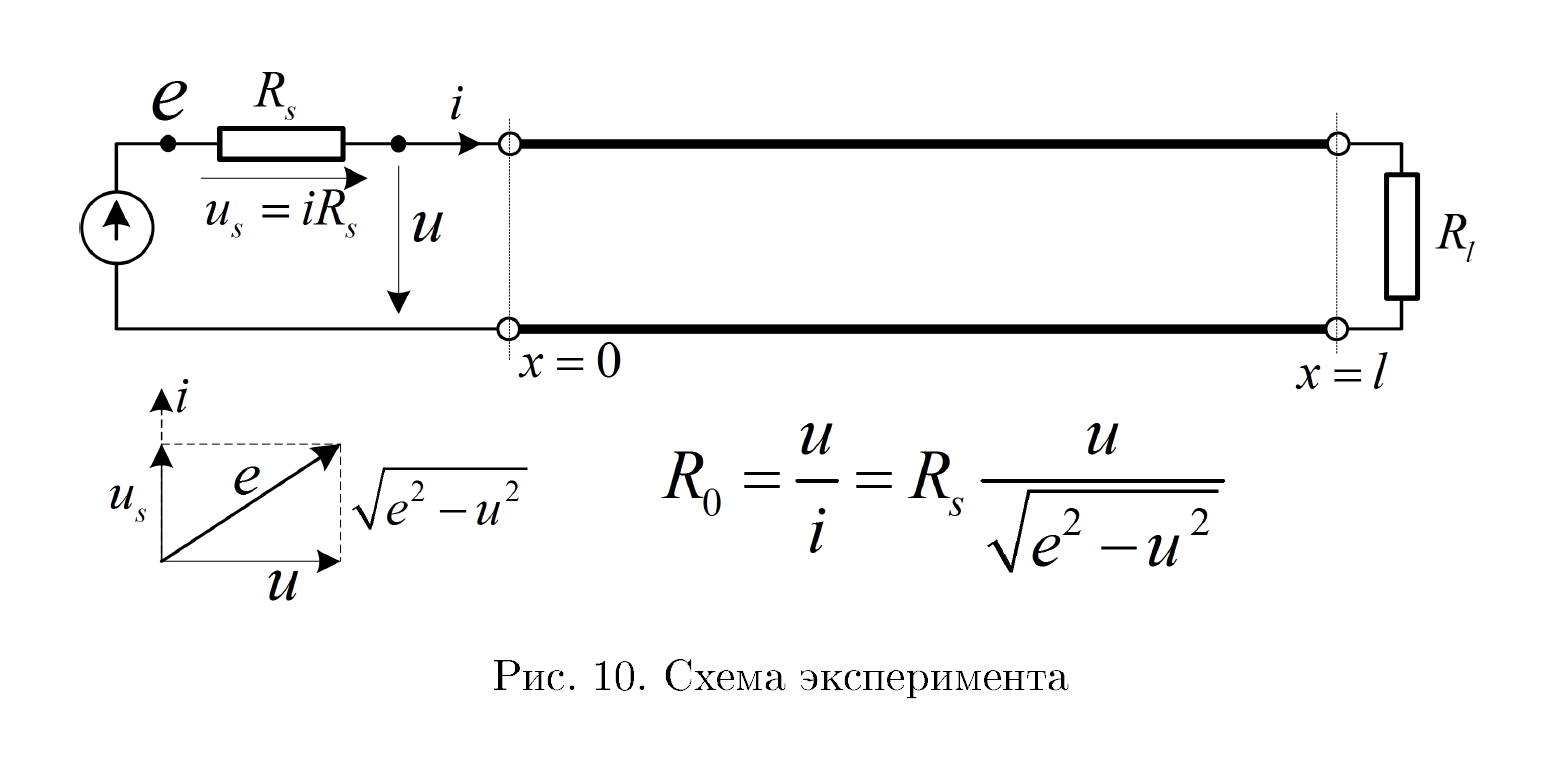
\includegraphics[width=0.95\textwidth]{схема.png}
	\label{fig:boiler}
\end{figure}

\subsubsection{Теория}

Измерения проводить на частоте f = 1.0-1.5 МГц при высоком уровне входного сигнала порядка 2-3 В. Эффективные значения напряжения источника e и напряжения на входе линии $u$ измерять параллельно двумя каналами осциллографа, используя входы с делением на 10. Имеет смысл предварительно проверить тождественность показаний в каналах и, при необходимости, ввести поправочный коэффициент. Для достижения достаточной точности измерений сопротивление источника $R_s$ подбирать так, чтобы напряжение $u$ на входе линии составляло порядка $\frac{e}{\sqrt{2}}$. В режиме короткого замыкания на выходе потребуется $R_s \simeq $ 30 - 50 Ом, в режиме холостого хода - $R_s \simeq$ 250 - 400 Ом.

Для вычисления входного сопротивления линии $R_0$ по измеренным значениям $e$ и $u$ использовать приведенную на рис формулу, которая учитывает факт ортогональности напряжений $u_s$ и $u$ на резисторе $R_s$ и входе линии следствие мнимости входного импеданса линии в отсутствие потерь.

\subsubsection{Выполнение}

1) Длина кабеля составляет $L = 5.9$ метра.

2) Используем сопротивления для короткого замыкания и холостого хода

\begin{equation}
	R_{s0} = 29 \text{ Ом}
\end{equation}

\begin{equation}
	R_{s \infty} = 352 \text{ Ом}
\end{equation}

Частота генератора $f = 1$ МГц.

Для короткого замыкания($R_{s0}$), $e = 3.09$ Вольта, $u = 1.955$ Вольта. Тогда

\begin{equation}
	R_0 = R_{s0} \frac{u}{\sqrt{e^2 - u^2}} = 287 \text{ Ом}
\end{equation}

Для холостого хода($R_{s0}$), $e = 3.09$ Вольта, $u = 1.855$ Вольта. Тогда

\begin{equation}
	R_{\infty} = R_{s\infty} \frac{u}{\sqrt{e^2 - u^2}} = 21.8 \text{ Ом}
\end{equation}

3) Волновое сопротивление линии

\begin{equation}
	\omega = \sqrt{\frac{L}{C}} = \sqrt{R_0 \cdot R_{\infty}} = 79 \text{ Ом}
\end{equation}

Скорость распространения волны

\begin{equation}
	v = \frac{1}{\sqrt{L C}} \approx 2 \pi f l \frac{\omega}{R_0} = 0.45 c
\end{equation}

Погонные емкость и индуктивность

\begin{equation}
	С = \frac{1}{\omega v} = 9.42 \cdot 10^{-11} \text{ Ф}
\end{equation}

\begin{equation}
	L = \frac{\omega}{v} = 5.88 \cdot 10^{-7} \text{ Гн}
\end{equation}

4) Исследуем резонансный пик на частоте $f_0 = 7.4$ МГц и $R_s = 1.1$ кОм. Тогда сопротивление

\begin{equation}
	R_0 = R_s \frac{u}{e - u} = 1 \text{ кОм}
\end{equation}

Ширина в результате

\begin{equation}
	\Delta f = 0.75 \text{ МГц}
\end{equation}

5) Погонное сопротивление

\begin{equation}
	R = \frac{\omega^2}{R_0 l} = 0.9 \text{ Ом}
\end{equation}

, что неплохо согласуется с прямым замером мультиметром.

Добротность

\begin{equation}
	Q = \frac{f_0}{\Delta f} \left( 1 + \frac{R_0}{R_s} \right) \approx 10
\end{equation}

Результат второй формулы $Q = \frac{\pi}{4}\frac{\omega}{R l}$ эквивалентен полученному.

Шунтирование ожидаемо расширяет полосу пропускания в $\simeq 1.9$ раз.

\subsubsection{Вывод}

\subsection{Исследование переходных процессов}

\begin{figure}[!h]
	\centering
	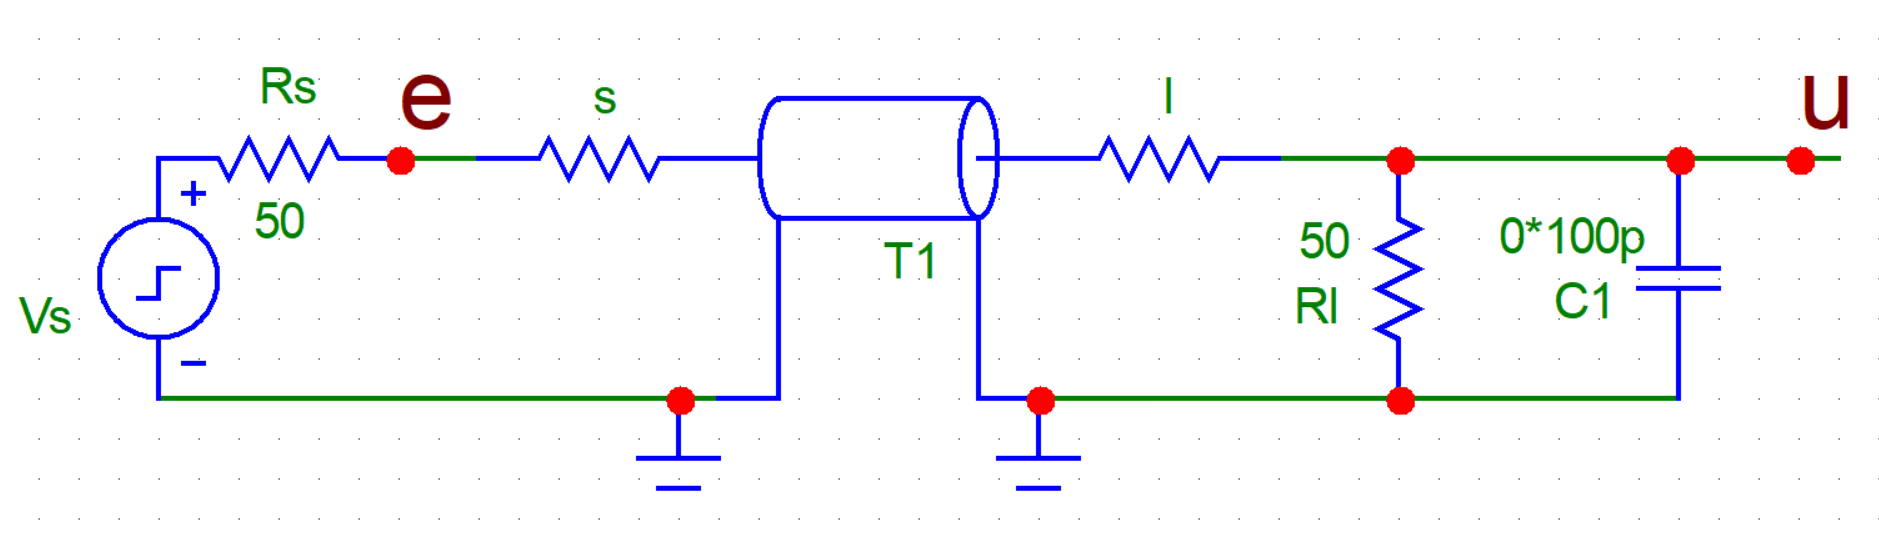
\includegraphics[width=0.95\textwidth]{модель.png}
	\label{fig:boiler}
\end{figure}

\subsubsection{Теория}

Исследования проводятся в режиме Transient MicroCap.

\subsubsection{Выполнение. Согласованная линия}

На схеме установим $R_s = R_l = 50$ Ом и выведем график в режиме \textit{Transient}.

\begin{figure}[h!]
\centering
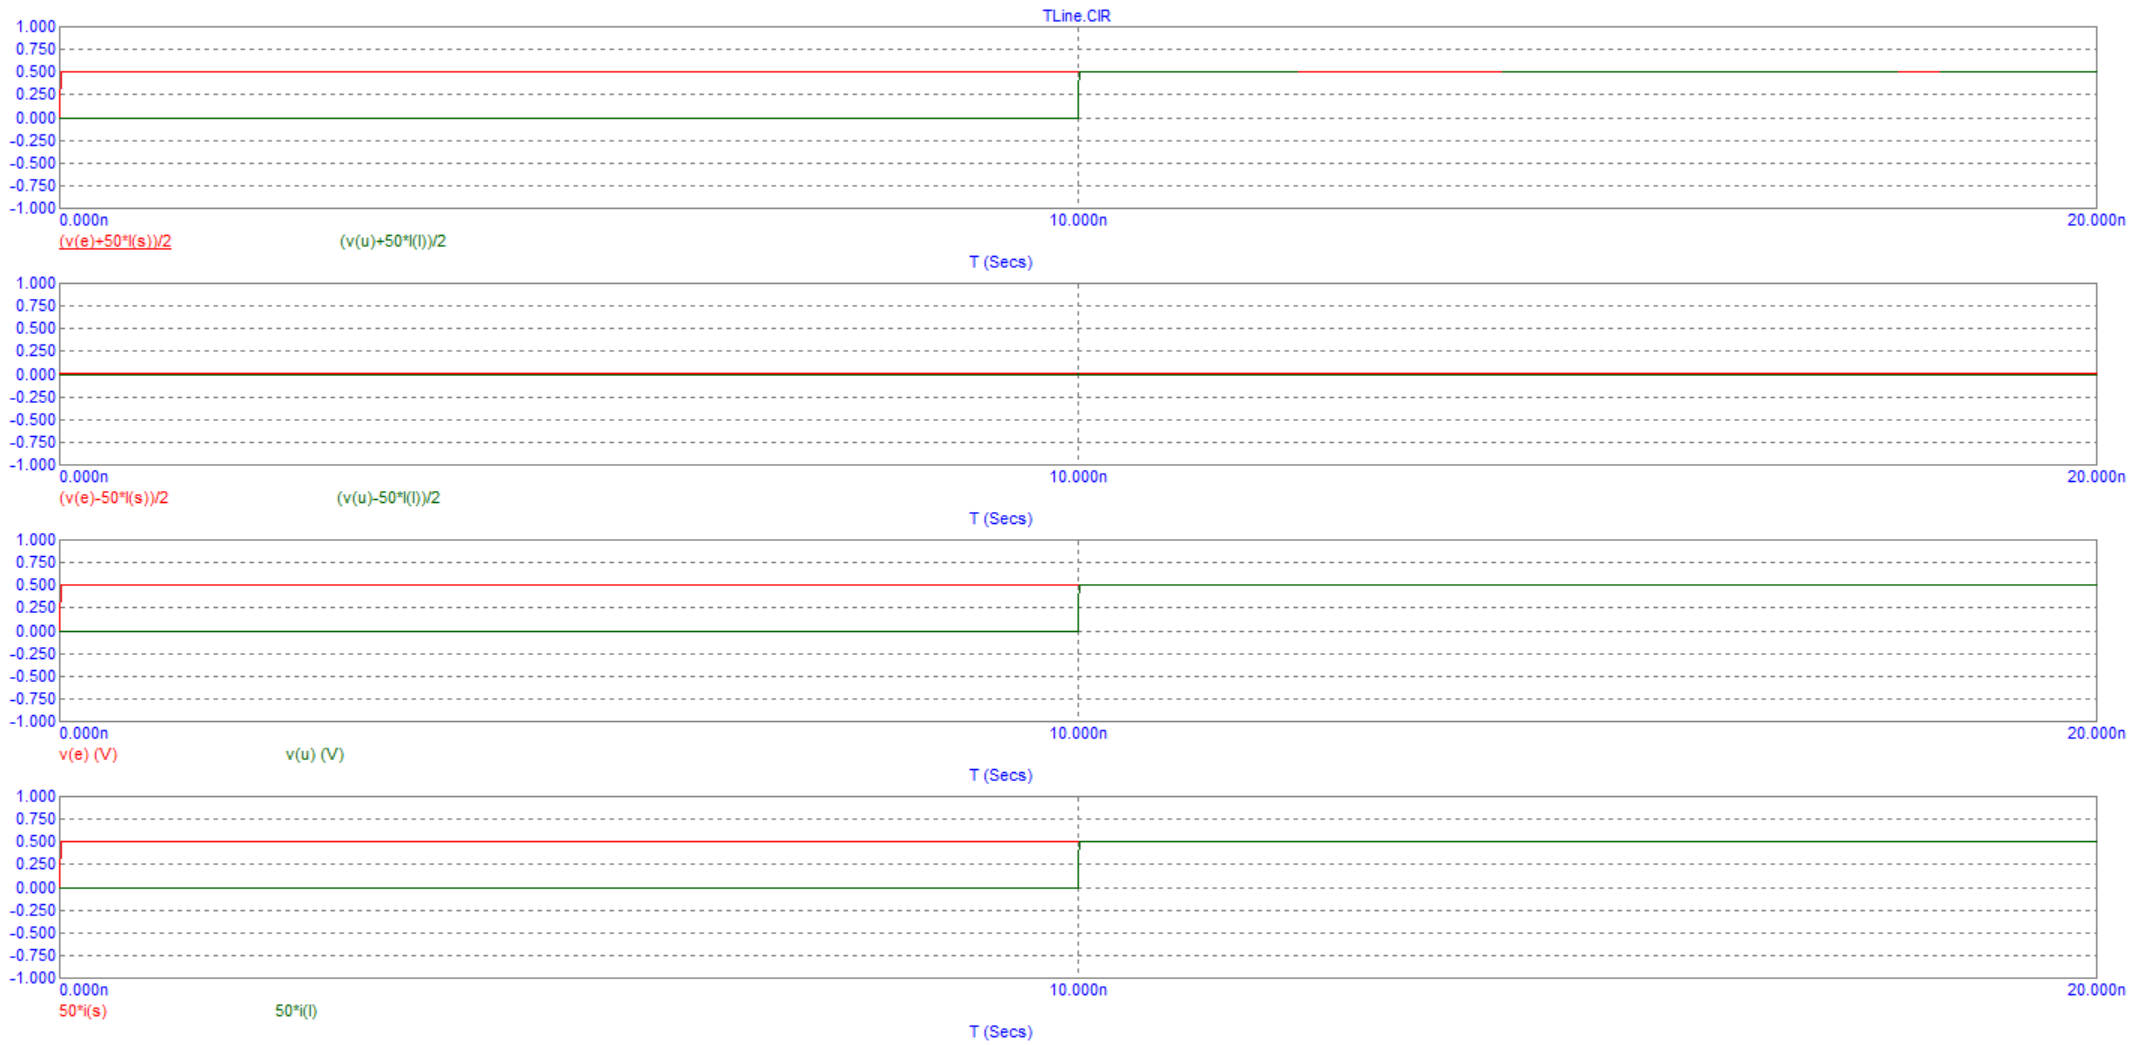
\includegraphics[width=0.95\textwidth]{картинки/Graph1.png}
\label{fig:Image1}
\end{figure}

Проанализируем графики и получим: $v(u) = 0.5 \: \textit{В}$ и $i(l)\cdot \omega = 0.5 \: \textit{В}$. Убедимся, что источник отражает предельную мощность

\[P = v(u)i(l) = \frac{V^2}{4R_s}, \: \text{где} \: V = 1\textit{ В}\]

\[P\omega = v(u)i(l)\omega = 0.5\cdot 0.5 = 0.25 = \frac{V^2}{4R_s} \omega,\]

Источник отражает предельную мощность.

\subsubsection{Рассогласованный источник}

Установим $R_s = \frac{\omega}{3} = \frac{50}{3} \: \textit{Ом}$. Выведем график в режиме \textit{Transient}.

\begin{figure}[h!]
\centering
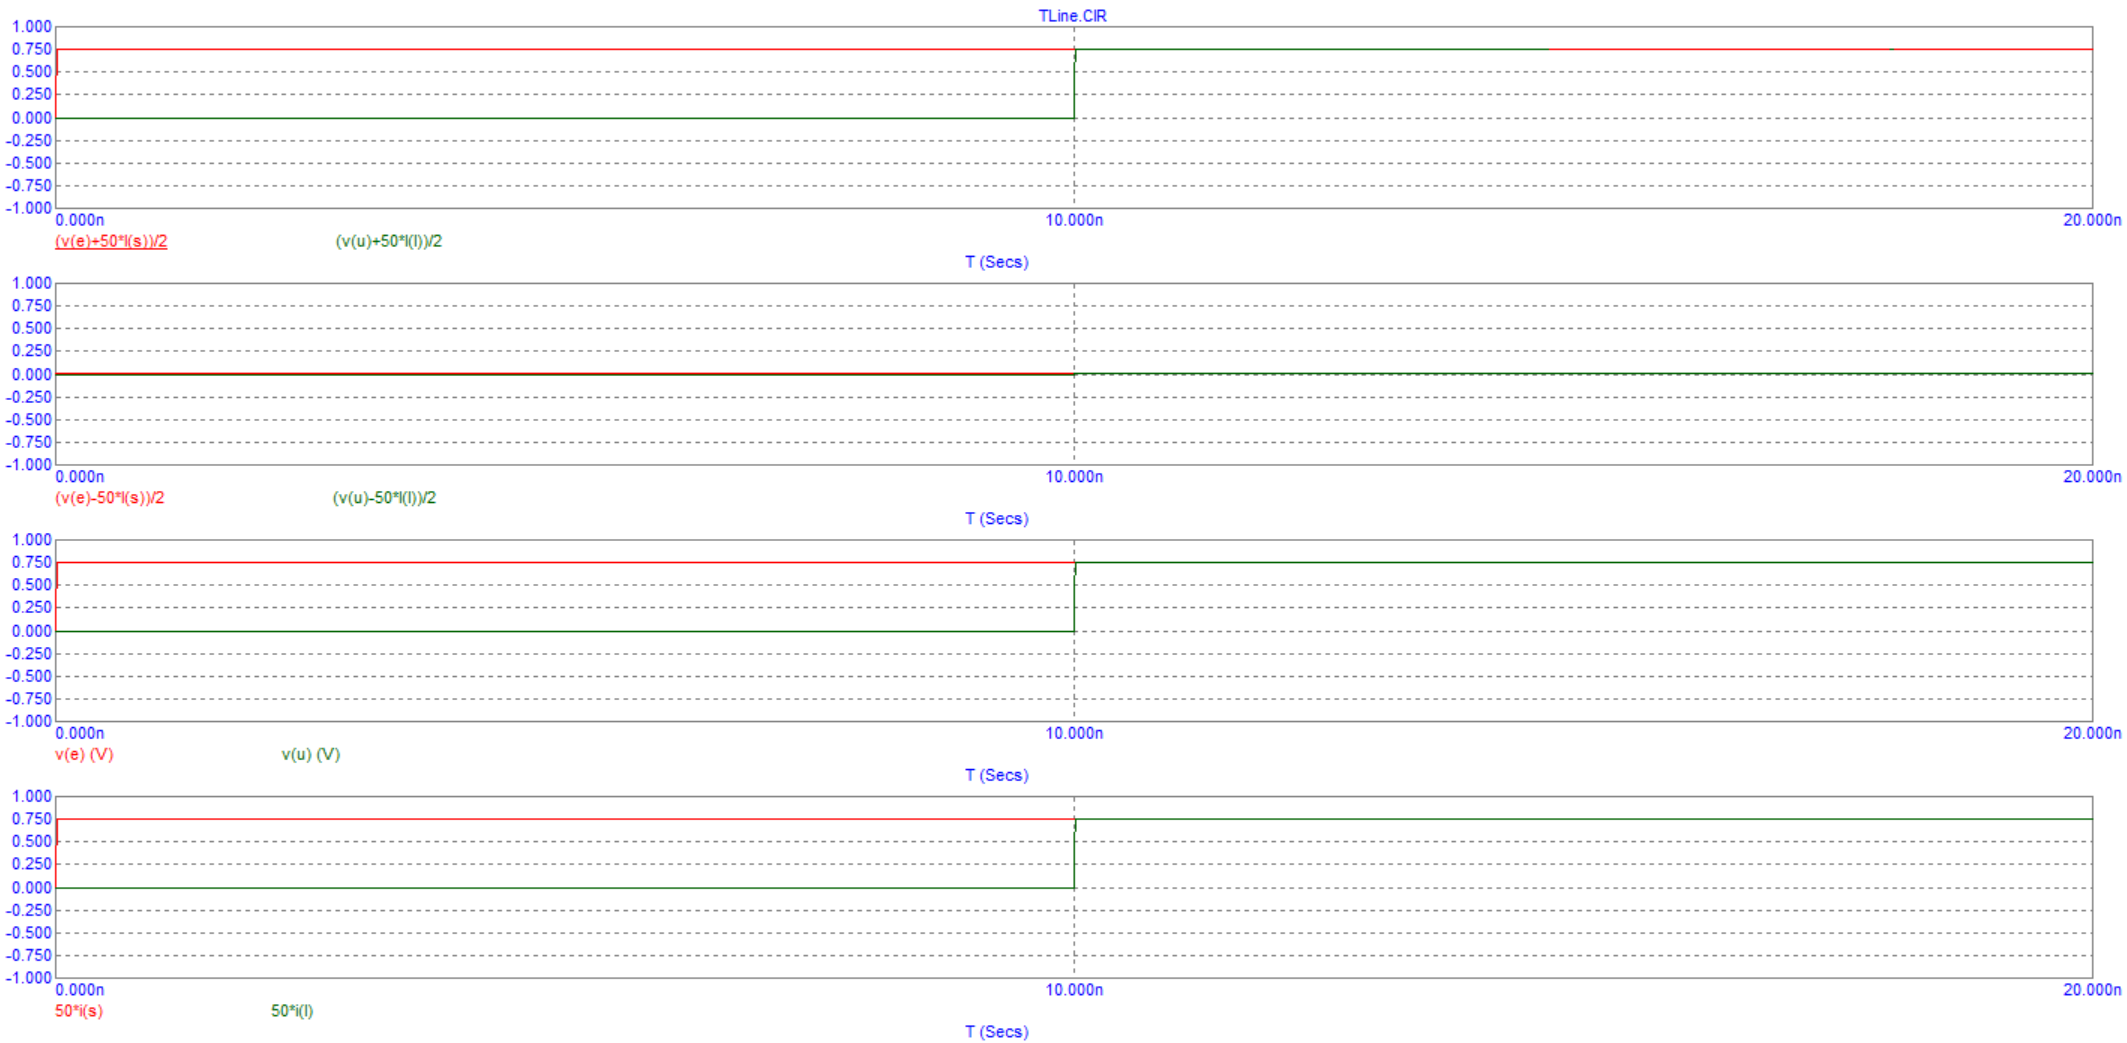
\includegraphics[width=0.95\textwidth]{картинки/Graph2.png}
\label{fig:Image1}
\end{figure}

Проанализируем графики и получим: $u(v) = 0.75 \: \textit{ В}$ и $i(l)\cdot \omega = 0.75 \: \textit{ В}$. Проверим, что отдаваемая мощность \textit{P} меньше мощности источника в $(1 - \rho_s^2)$ раз:

\[\rho_s = \frac{R_s - \omega}{R_s + \omega} = -\frac{1}{2}\]

\[P\omega = v(u)i(l)\omega = 0.75 \cdot 0.75 = 0.5625 = \frac{V^2}{4R_s} \omega (1 - \rho_s^2),\]

Повторим все это при $R_s = 3\omega = 150 \: \textit{ Ом}$

\begin{figure}[h!]
\centering
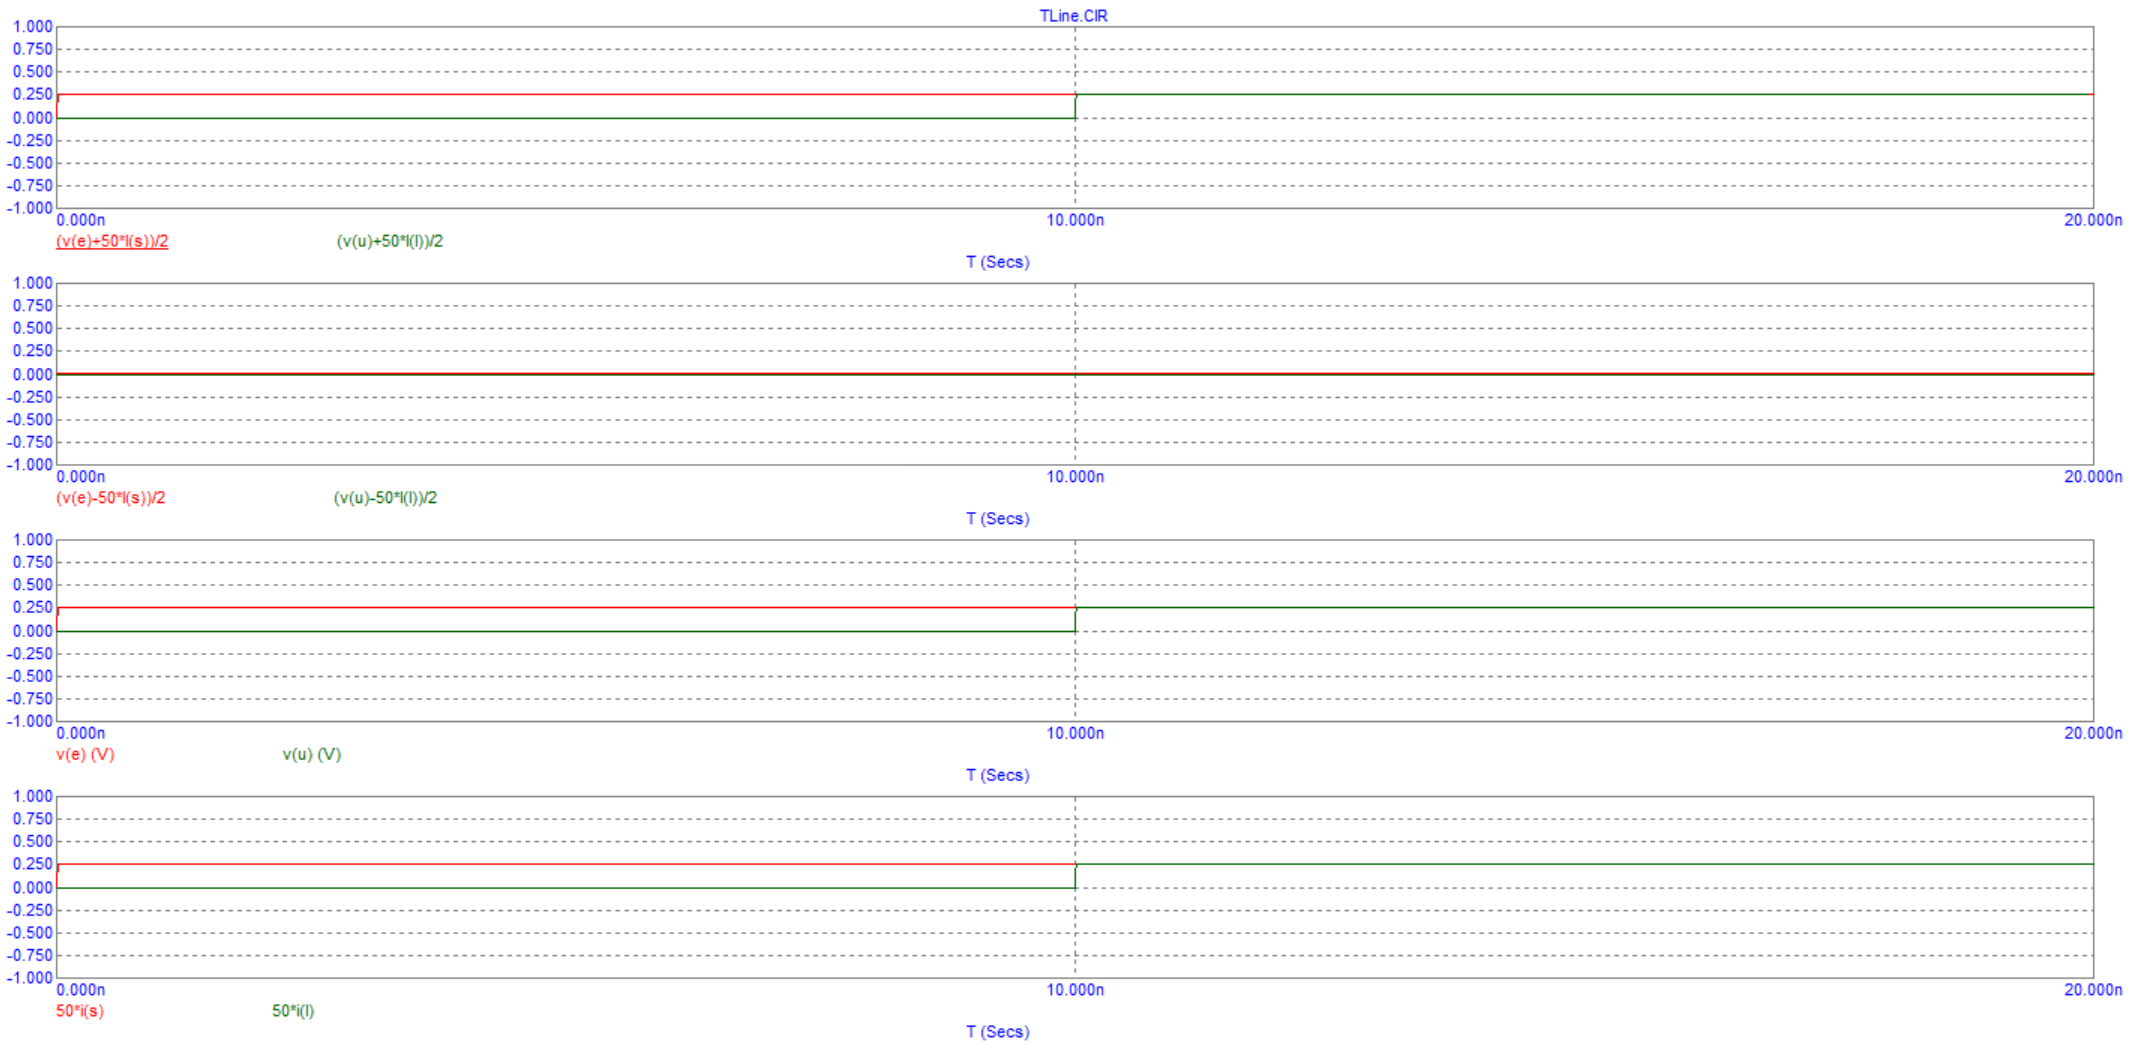
\includegraphics[width=0.95\textwidth]{картинки/Graph3.png}
\label{fig:Image1}
\end{figure}

Проанализируем графики и получим: $u(v) = 0.25 \: \textit{В}$ и $i(l)\cdot \omega = 0.25 \: \textit{ В}$. Проверим, что отдаваемая мощность \textit{P} меньше мощности источника в $(1 - \rho_s^2)$ раз:

\[\rho_s = \frac{R_s - \omega}{R_s + \omega} = \frac{1}{2}\]

\[P\omega = v(u)i(l)\omega = 0.25 \cdot 0.25 = 0.0625 = \frac{V^2}{4R_s} \omega (1 - \rho_s^2)\]

Равенства справедливы.

\subsubsection{Рассогласованная нагрузка}

Установим варьированием $R_l = \frac{\omega}{3} = \frac{50}{3} \: \textit{ Ом}$ $[\rho_l = - \frac{1}{2}]$, $R_l = 0 \: \textit{ Ом}$ $[\rho_l = 0]$, $R_l = 3\omega = 150 \: \textit{ Ом}$, $[\rho_l =  \frac{1}{2}]$ $R_l = \frac{\omega}{3} = 50 \: \textit{ кОм}$ $[\rho_l =  +1]$ ($R_s = 50 \textit{ Ом}$). Измерим установившиеся значения амплитуд волн, напряжений и токов.

\begin{figure}[h!]
\centering
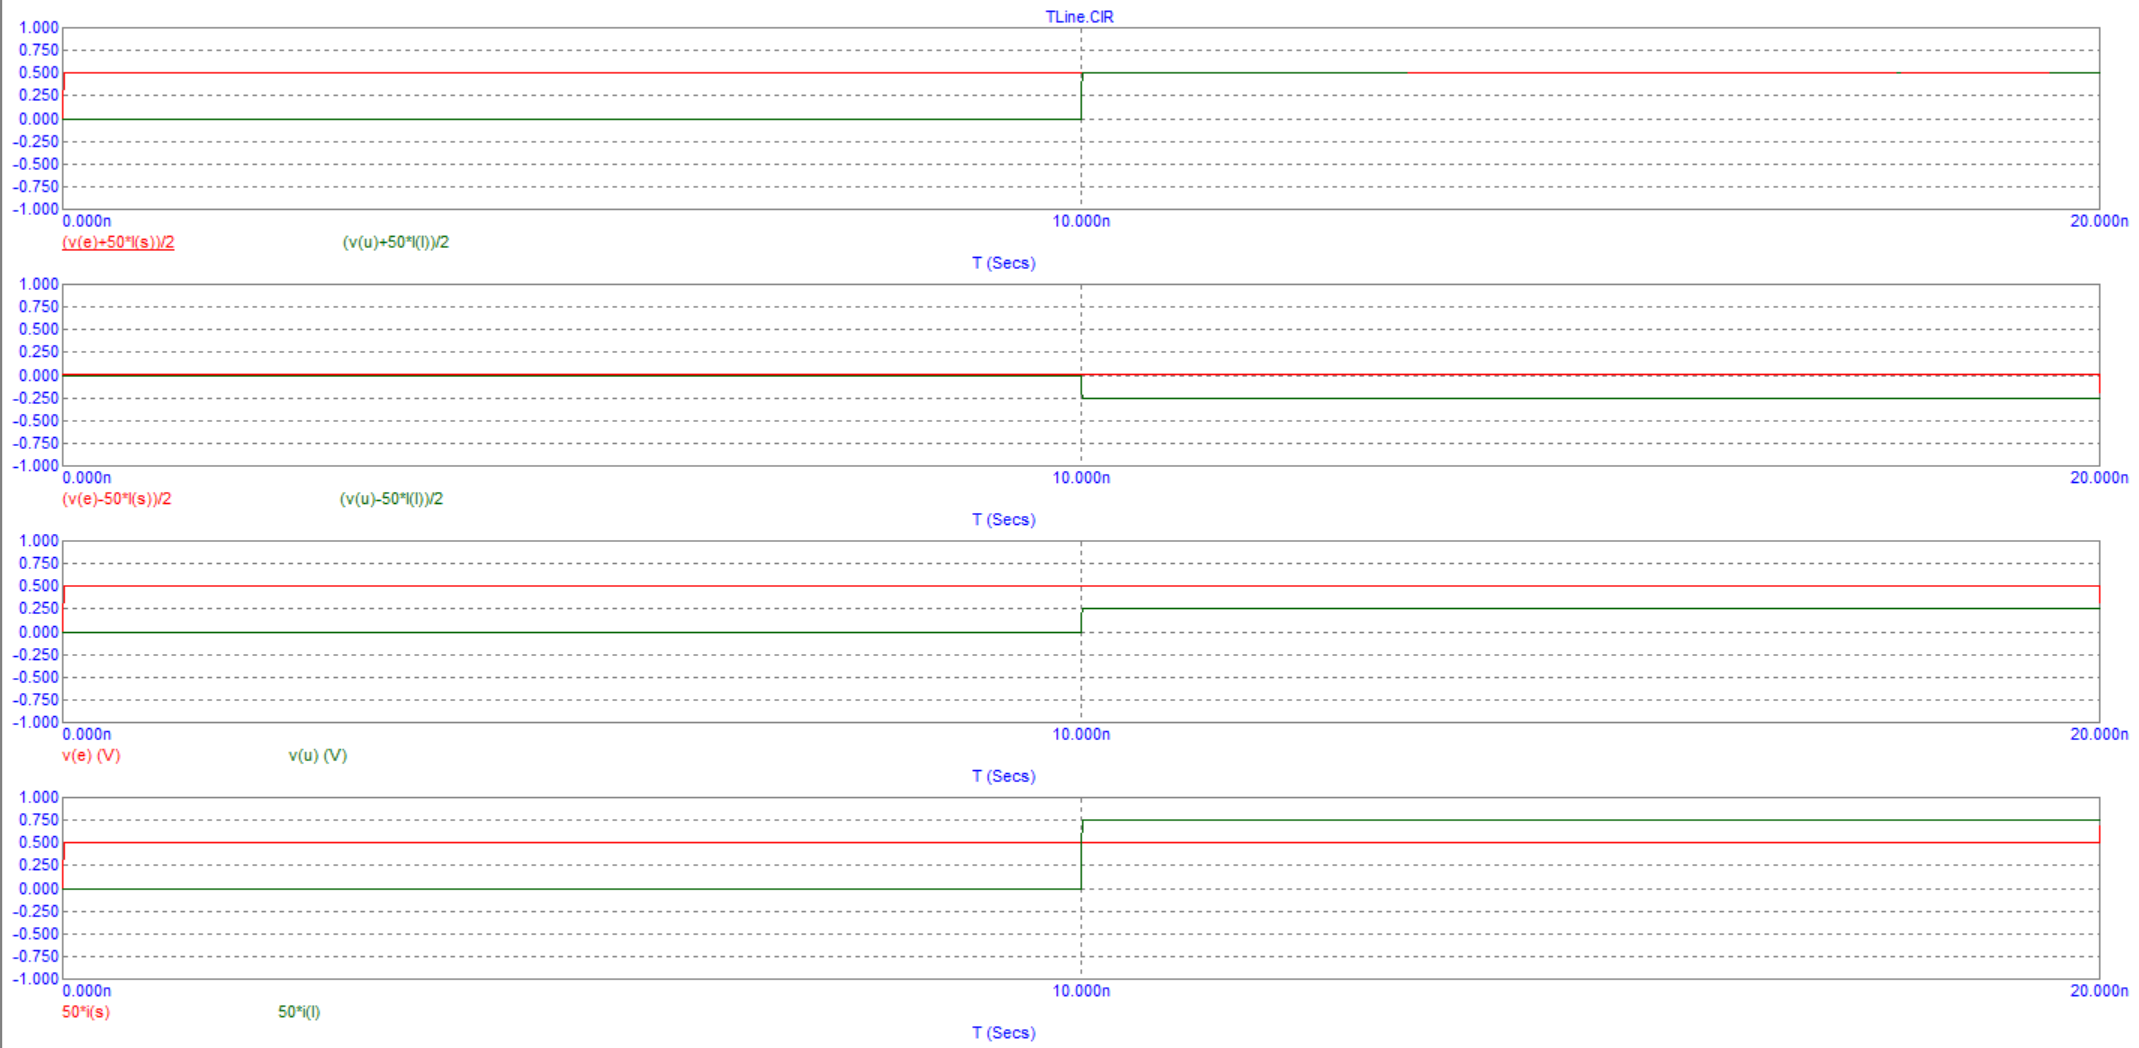
\includegraphics[width=0.95\textwidth]{картинки/Graph4.png}
\label{fig:Image1}
\caption{$R_l = \frac{\omega}{3}$}
\end{figure}

.

\begin{figure}[h!]
\centering
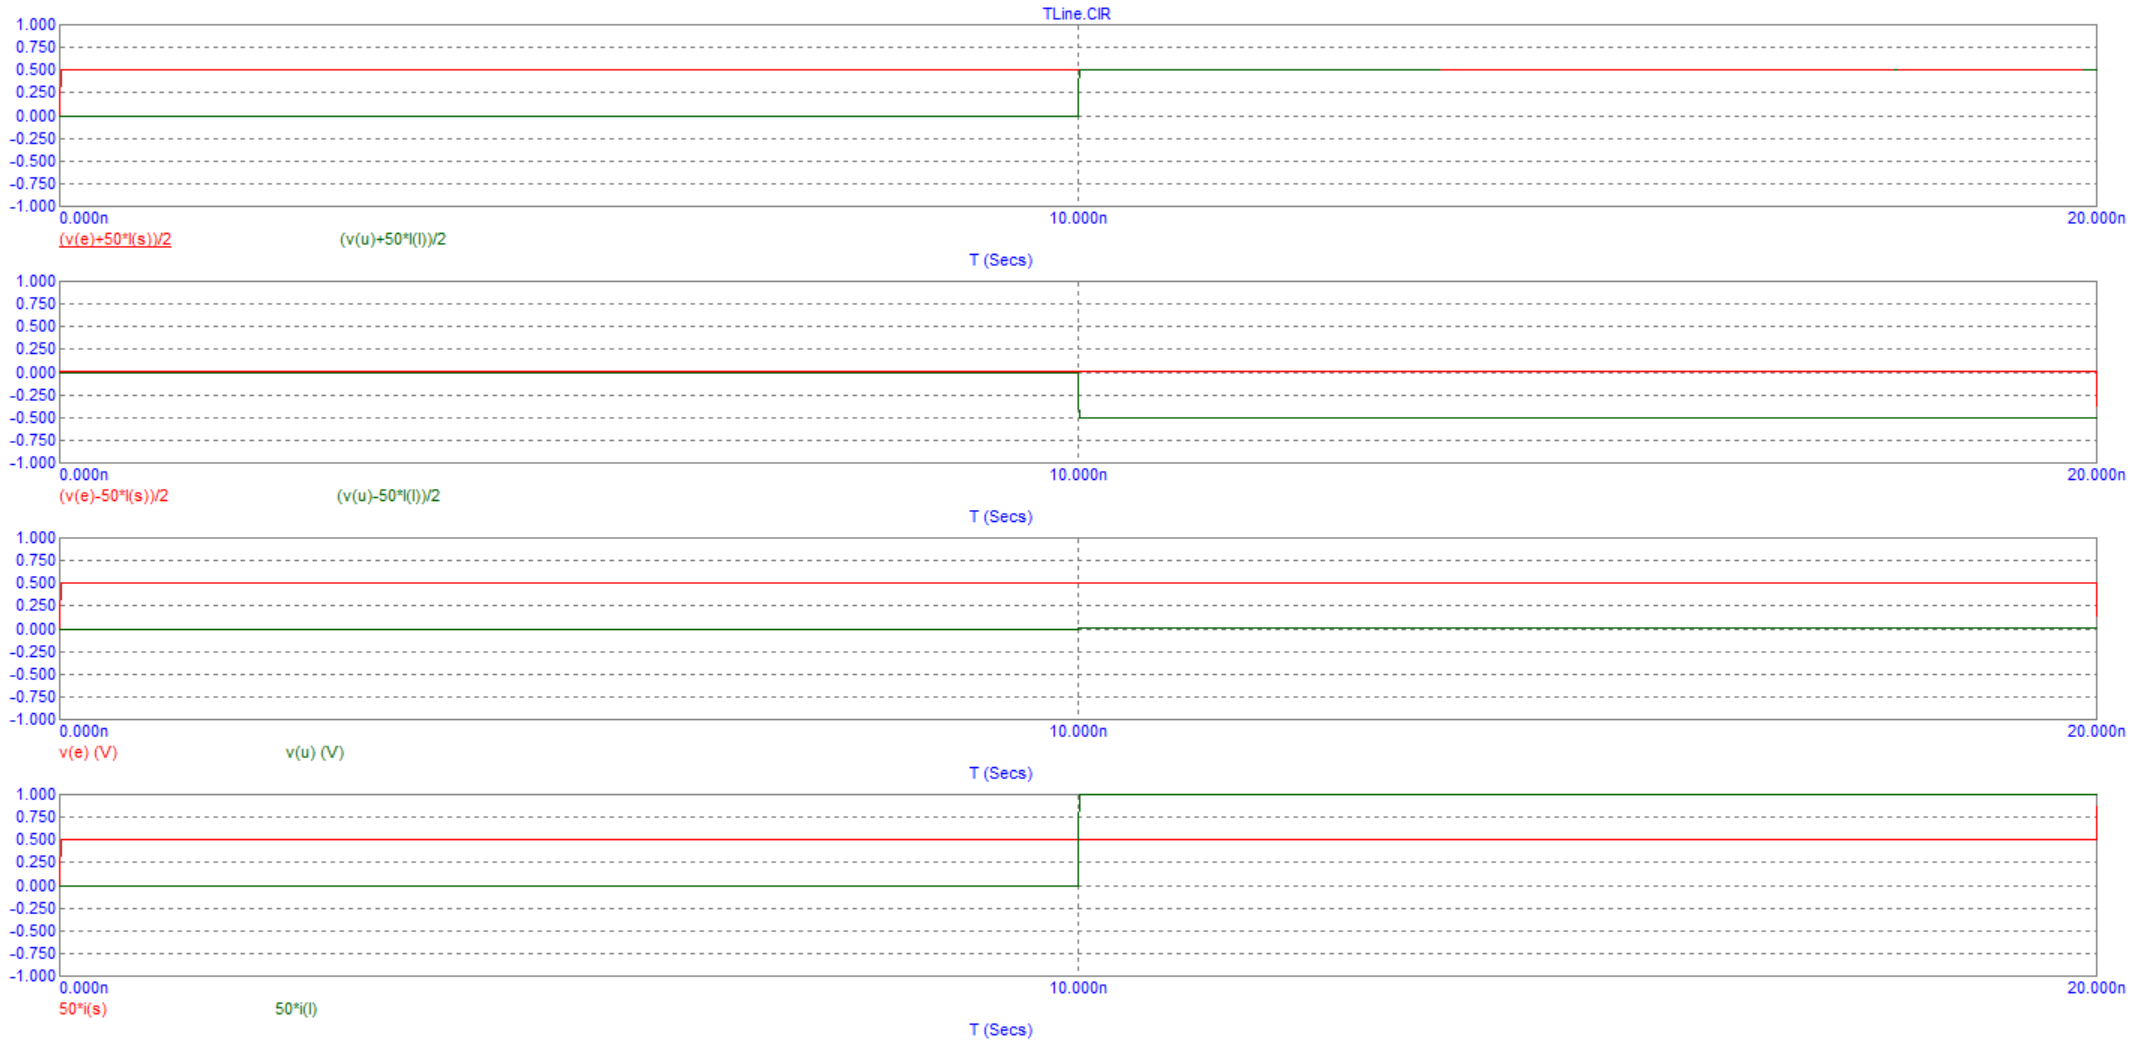
\includegraphics[width=0.95\textwidth]{картинки/Graph5.png}
\label{fig:Image1}
\caption{$R_l = 0$}
\end{figure}

\newpage

\begin{figure}[h!]
\centering
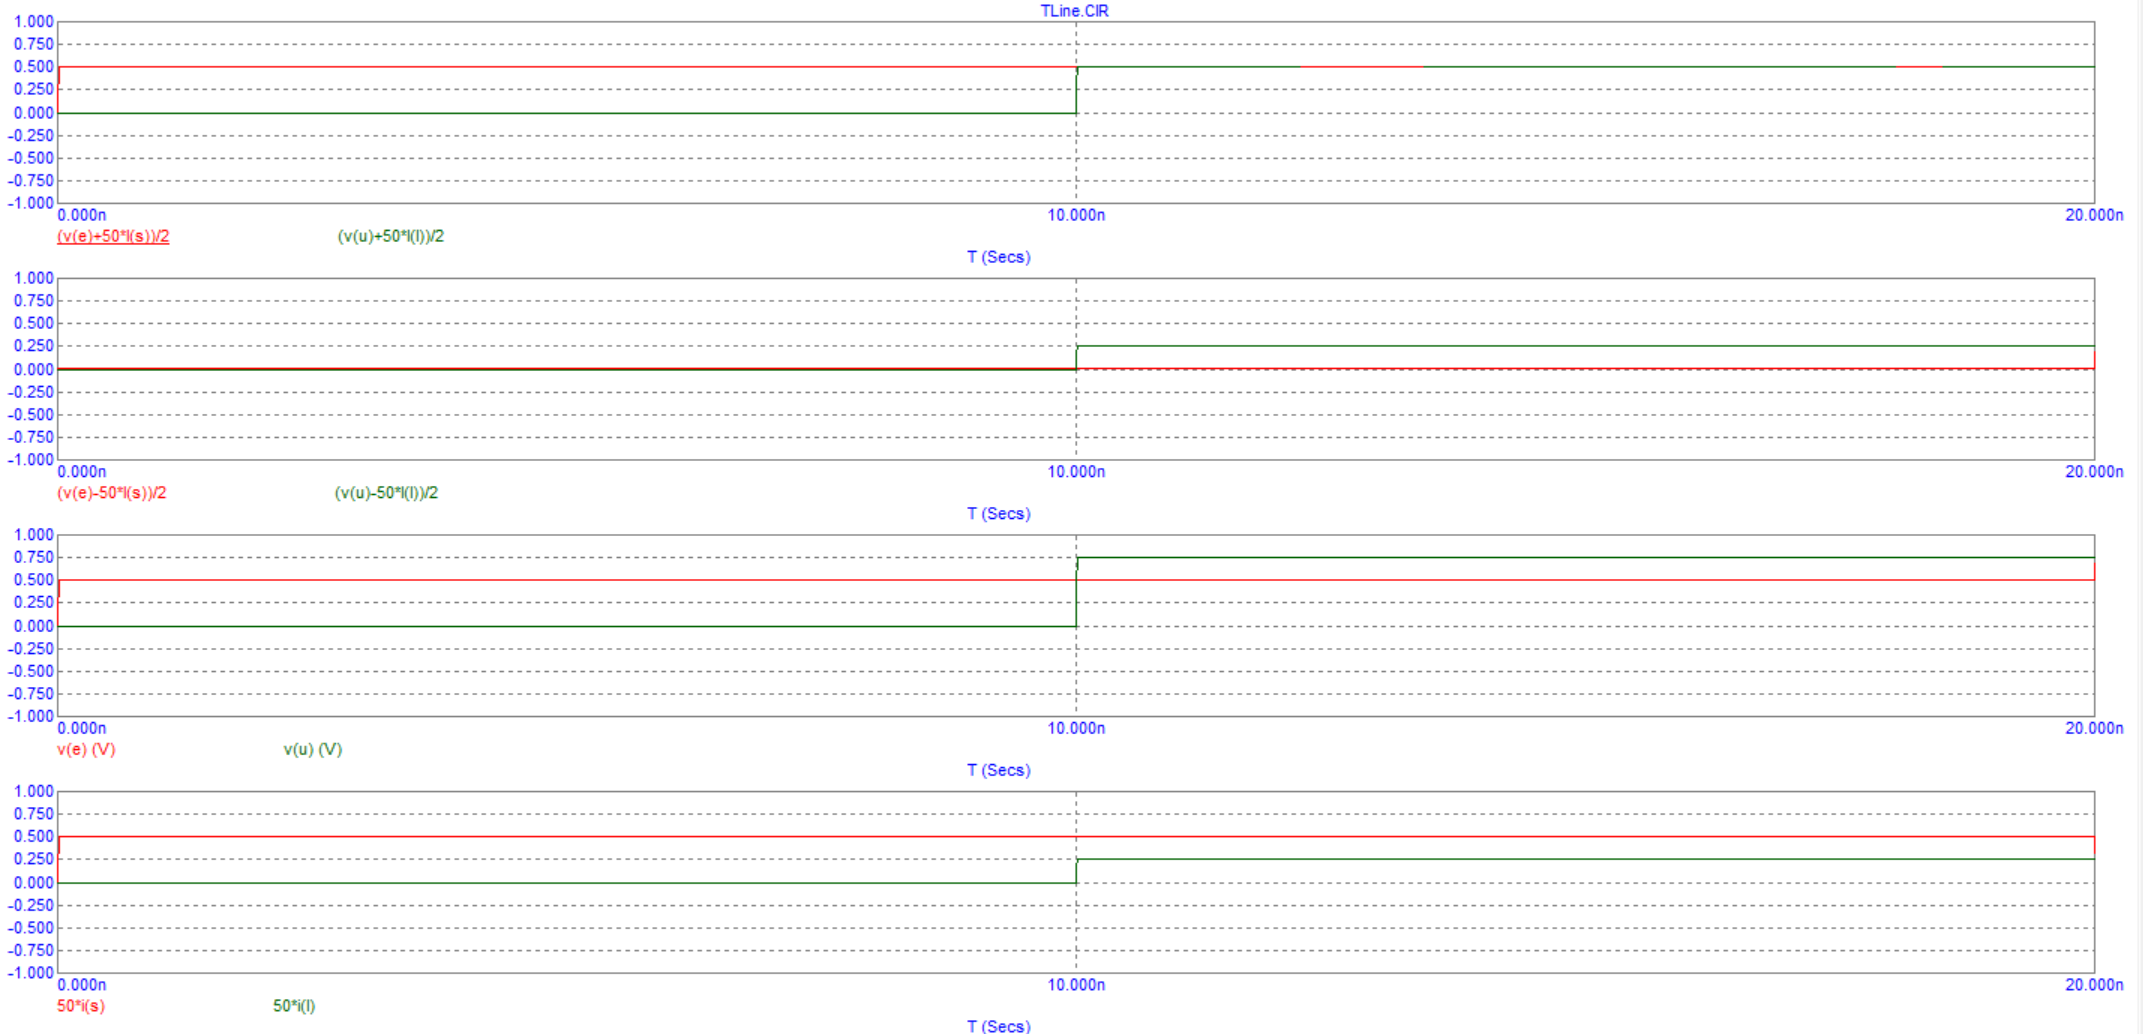
\includegraphics[width=0.95\textwidth]{картинки/Graph6.png}
\label{fig:Image1}
\caption{$R_l = 3\omega$}
\end{figure}

.

\begin{figure}[h!]
\centering
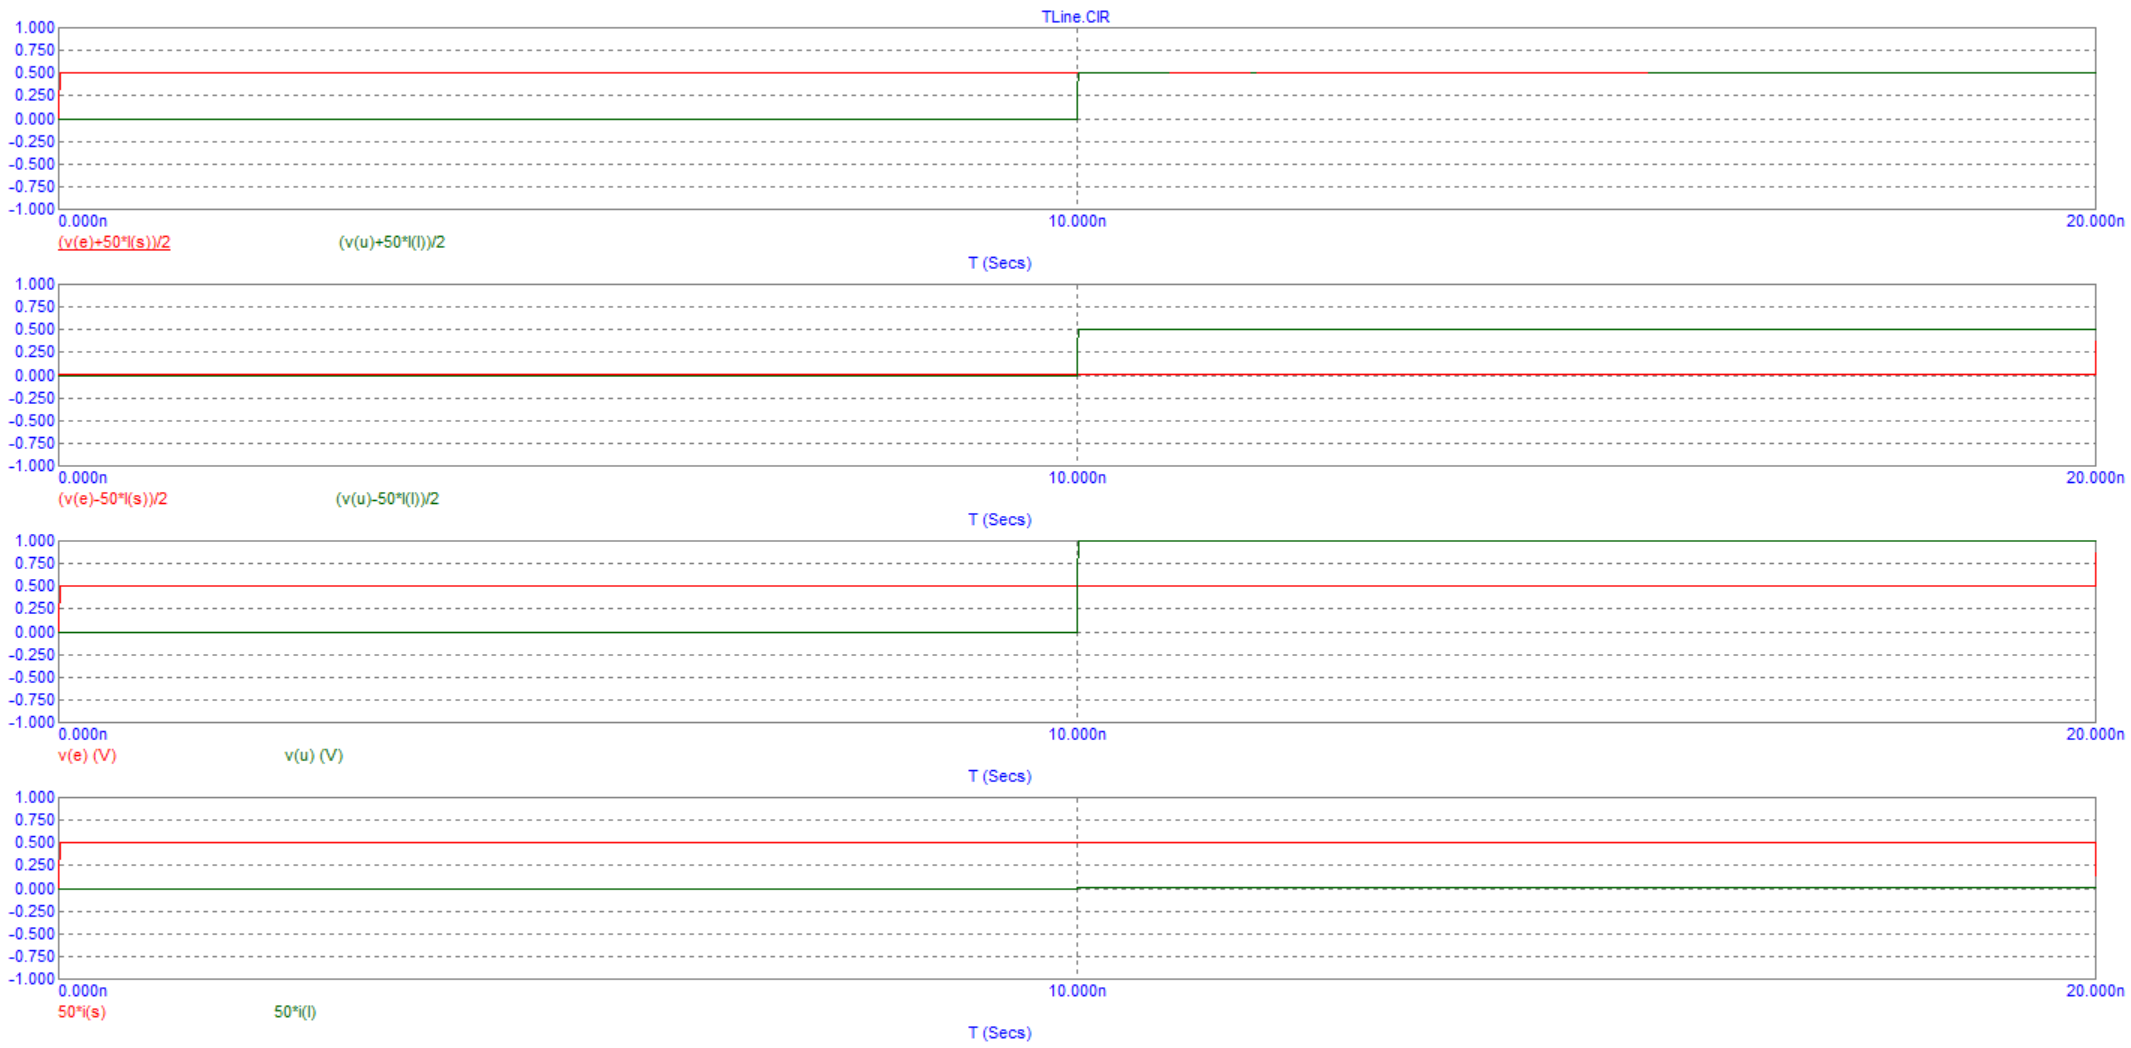
\includegraphics[width=0.95\textwidth]{картинки/Graph7.png}
\label{fig:Image1}
\caption{$R_l = 50k$}
\end{figure}

\newpage

Запишем данные в таблицу:

\begin{center}
\begin{tabular}{|c|c|c|c|c|}
\hline 
$R_l/\omega$ & 1/3 & 0 & 3 & $\infty$ \\ 
\hline 
A & 0.5 & 0.5 & 0.5 & 0.5 \\ 
\hline 
B & -0.25 & -0.5 & 0.25 & 0.5 \\ 
\hline 
$v(u)$ & 0.25 & 0 & 0.75 & 1 \\ 
\hline 
$i(l)\omega$ & 0.75 & 1 & 0.25 & 0 \\ 
\hline 
\end{tabular} 
\end{center}

\subsubsection{Рассогласованные источник и нагрузка}

Установим на схеме $R_s = 50/3 \: [\rho_s = -\frac{1}{2}]$. Установим варьированием $R_l = 0 \: [\rho_l = -1]$, $\rho_s \rho_l = \frac{1}{2}$, выведем графики.

\begin{figure}[h!]
\centering
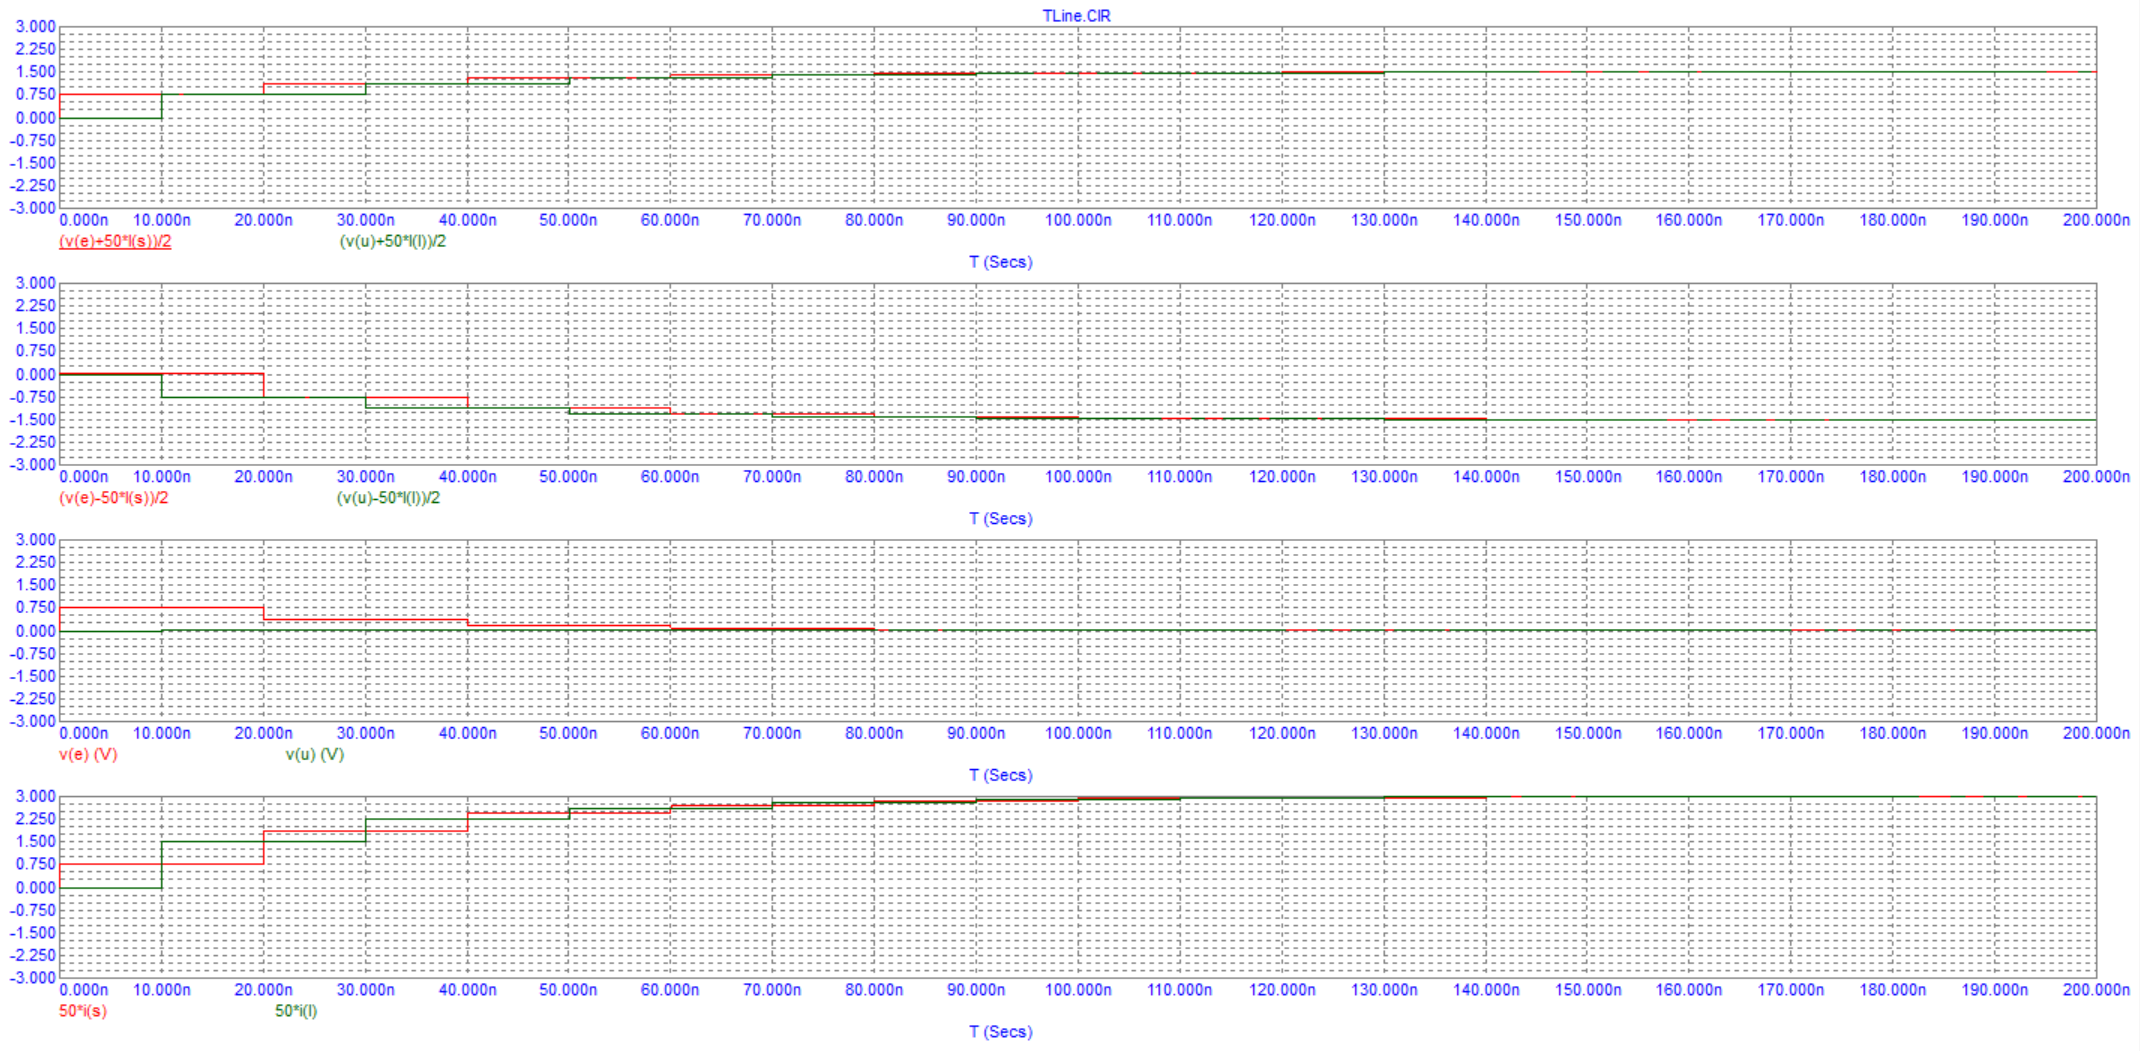
\includegraphics[width=0.95\textwidth]{картинки/Graph8.png}
\label{fig:Image1}
\caption{$R_l = 0, R_s = 50/3$}
\end{figure}

Убедимся в том, что амплитуда пдающей волны нарастает, как последовательных частичных сумм прогрессии:

\[A = \frac{\omega}{\omega + R_s} \Big( 1 + \rho_s \rho_l + (\rho_s \rho_l)^2 + ...\Big) = \frac{3}{4} \Big( 1 + \frac{1}{2} + \frac{1}{4} + ... \Big) = 1.5\]

Первый шаг $(n = 1): \: A = 0.75$.

Второй шаг $(n = 2): \: A = 1.125$.

Третий шаг $(n = 3): \: A = 1.3125$.

Установившееся значение: $(n = \infty): \: A = 1.5$.

\newpage

Повторим наблюдения при $R_l = 50k \simeq \infty \: [\rho_l = 1], \: \rho_s \rho_l = -\frac{1}{2}$:

\begin{figure}[h!]
\centering
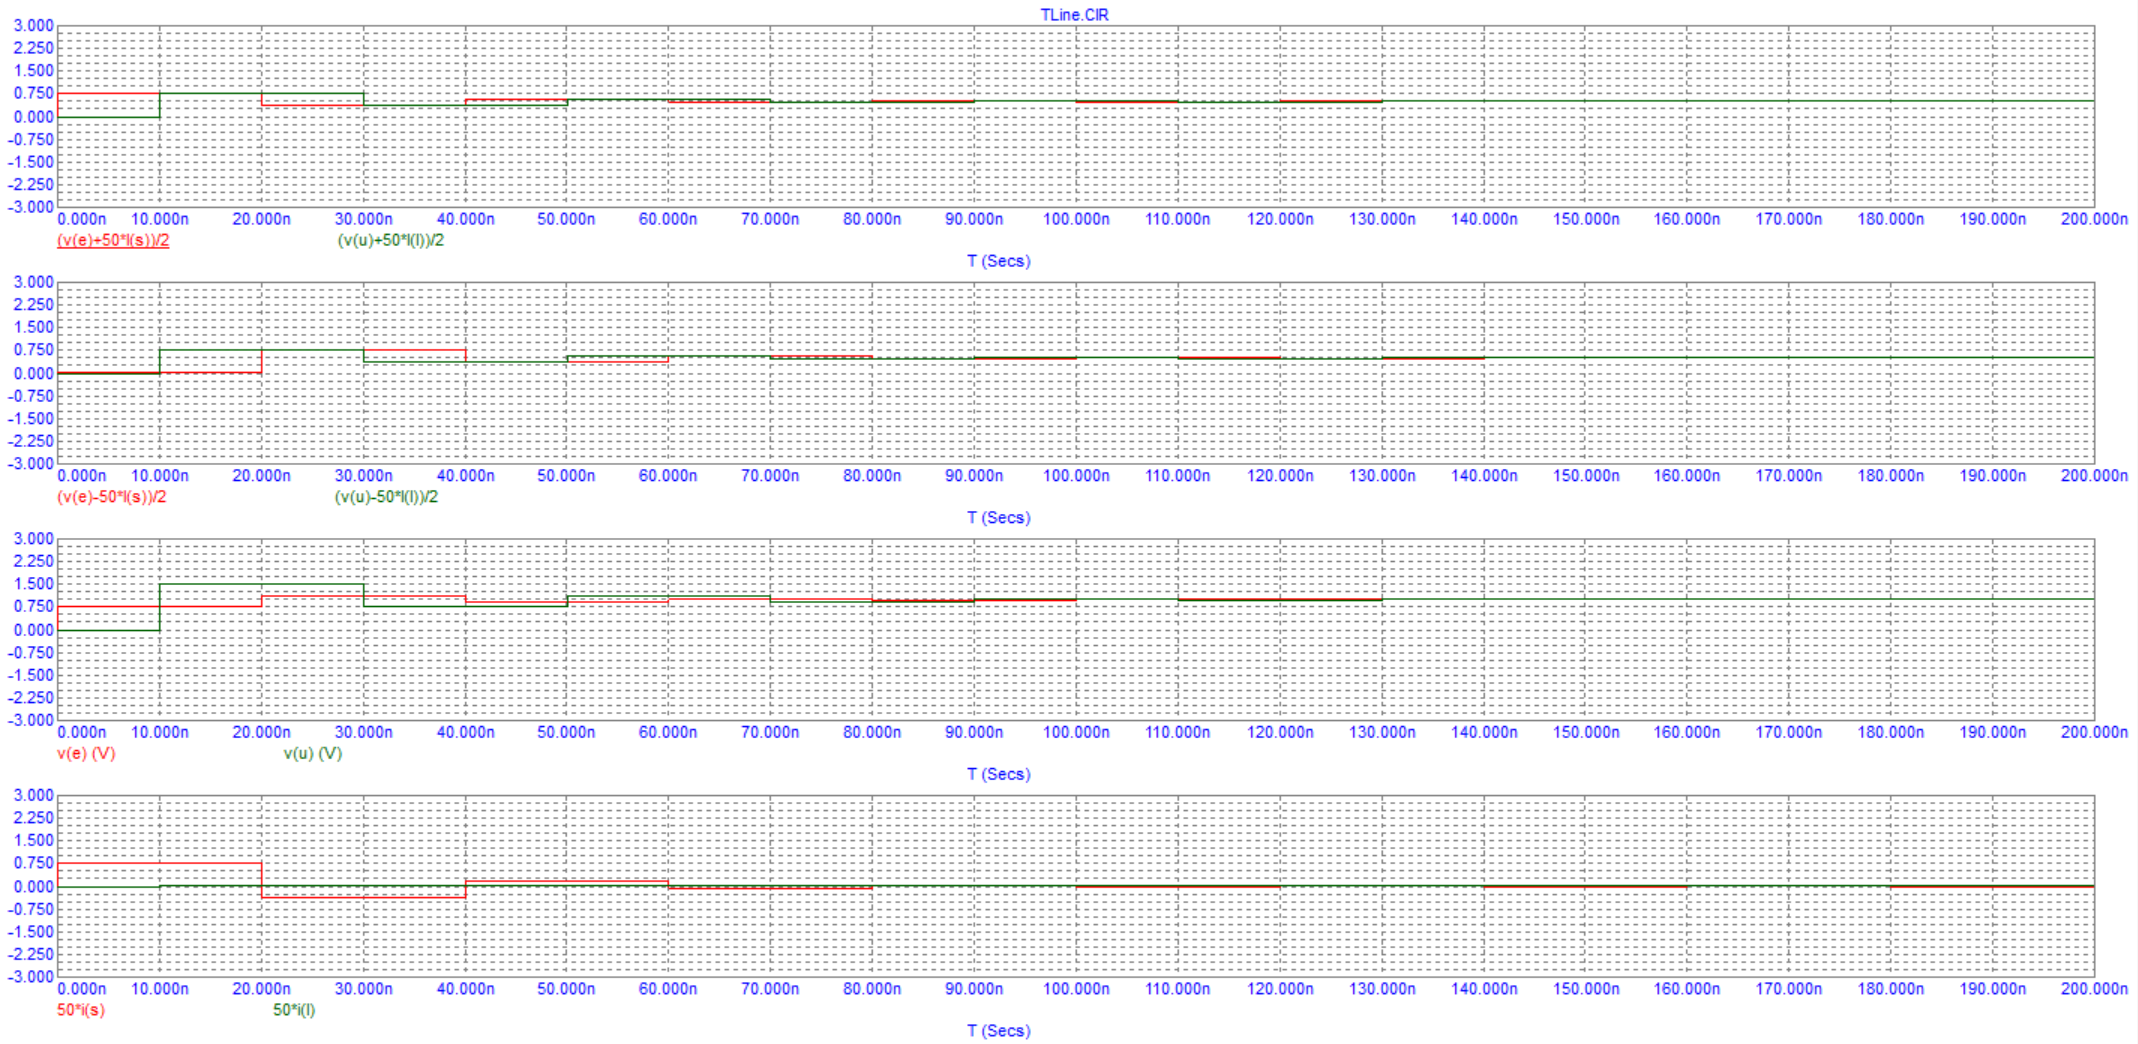
\includegraphics[width=0.95\textwidth]{картинки/Graph9.png}
\label{fig:Image1}
\caption{$R_l = 50k, R_s = 50/3$}
\end{figure}

\[A = \frac{\omega}{\omega + R_s} \Big( 1 + \rho_s \rho_l + (\rho_s \rho_l)^2 + ...\Big) = \frac{3}{4} \Big( 1 - \frac{1}{2} + \frac{1}{4} - ... \Big) = \frac{3}{4} \cdot \frac{2}{3} = \frac{1}{2}\]

Первый шаг $(n = 1): \: A = 0.75$.

Второй шаг $(n = 2): \: A = 0.375$.

Третий шаг $(n = 3): \: A = 0.5625$.

Установившееся значение: $(n = \infty): \: A = 0.5$.

\newpage

Установим на схеме $R_s = 50\omega \: [\rho_s = \frac{1}{2}]$ и повторим наблюдения при $R_l = 0 \:[\rho_l = -1]$.

\begin{figure}[h!]
\centering
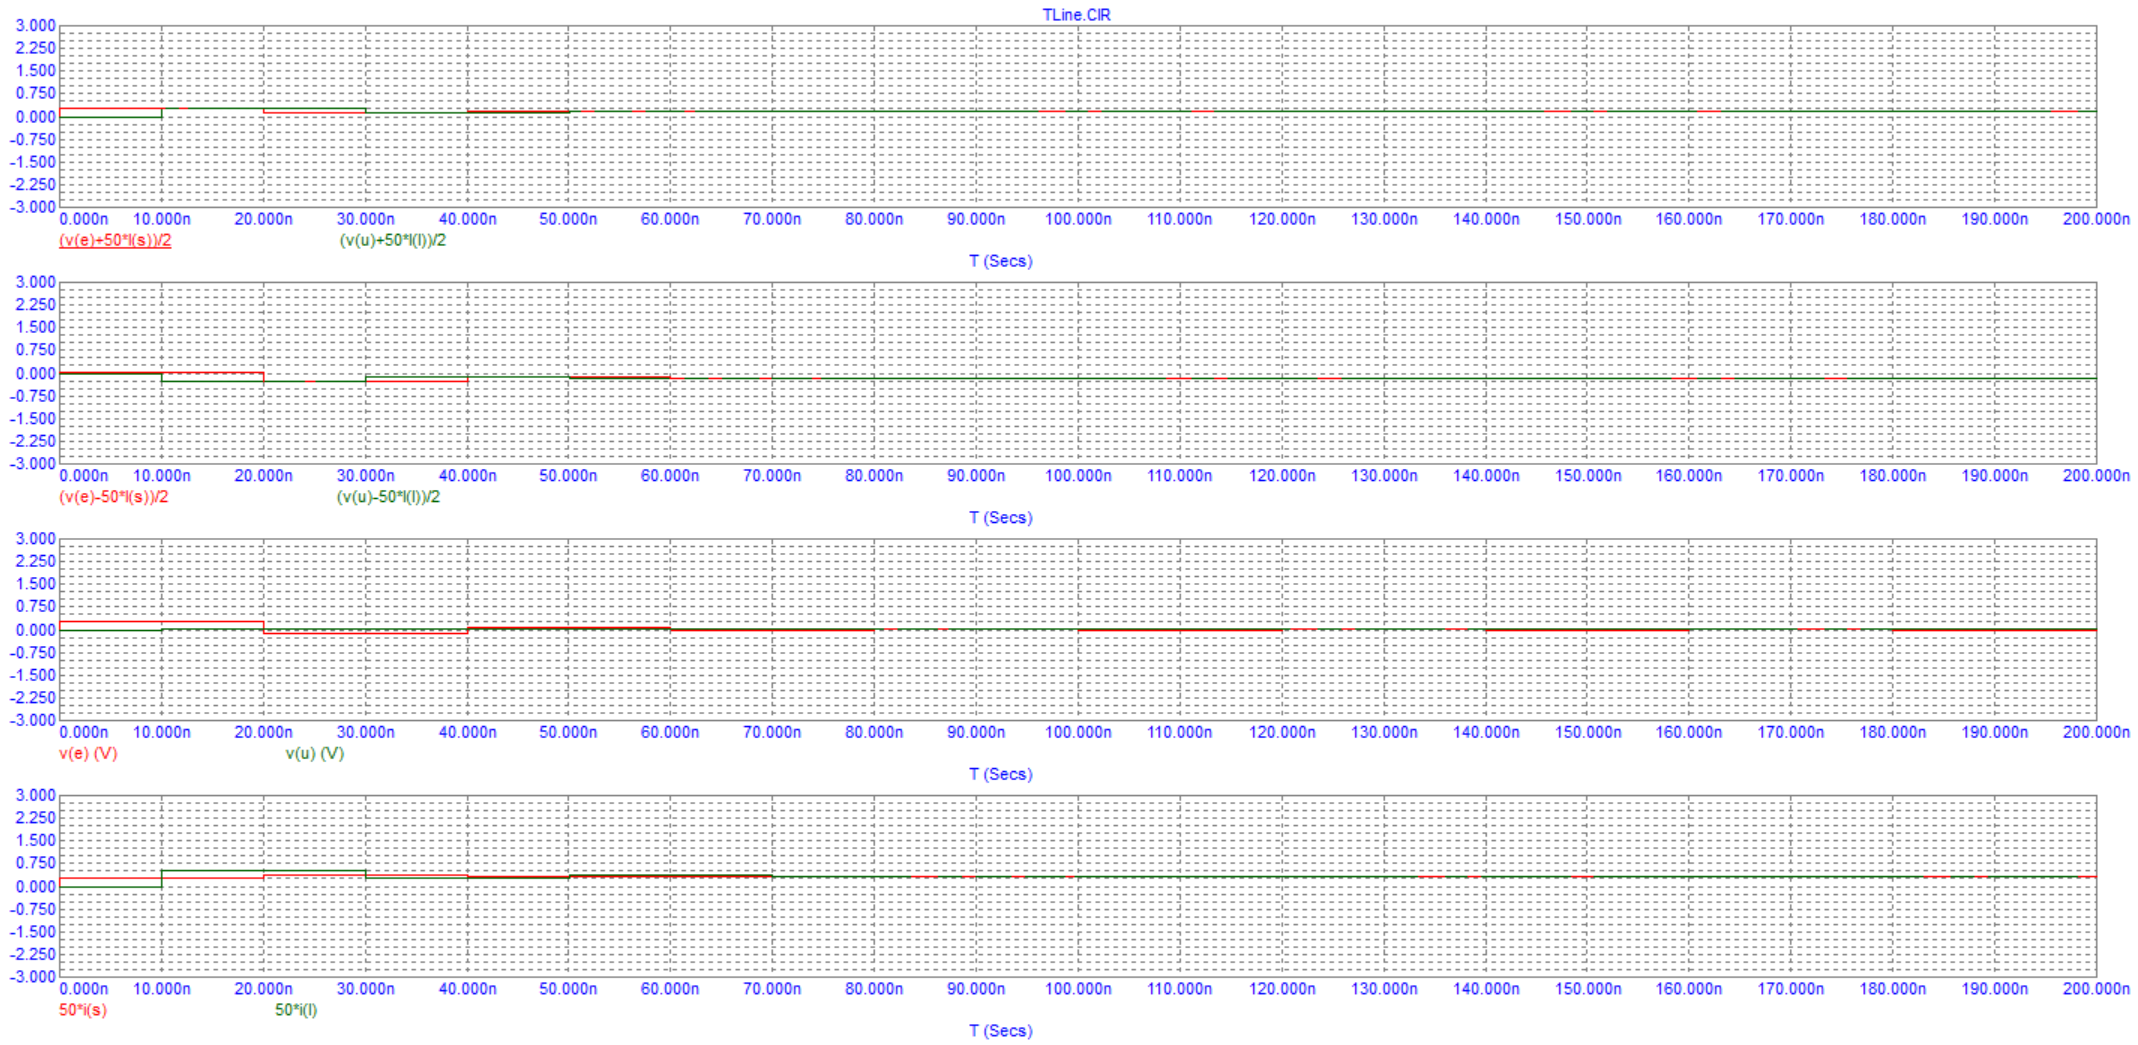
\includegraphics[width=0.95\textwidth]{картинки/Graph10.png}
\label{fig:Image1}
\caption{$R_l = 50k, R_s = 50/3$}
\end{figure}

\[A = \frac{\omega}{\omega + R_s} \Big( 1 + \rho_s \rho_l + (\rho_s \rho_l)^2 + ...\Big) = \frac{1}{4} \Big( 1 - \frac{1}{2} + \frac{1}{4} - ... \Big) = \frac{1}{4} \cdot \frac{2}{3} = \frac{1}{6}\]

Первый шаг $(n = 1): \: A = 0.25$.

Второй шаг $(n = 2): \: A = 0.125$.

Третий шаг $(n = 3): \: A = 0.1875$.

Установившееся значение: $(n = \infty): \: A = \frac{1}{6}$.

\newpage

Установить на схеме $R_s = 0 \: [\rho_s = -1]$ (предельно сильное рассогласование на источнике) и повторить наблюдения при

\[R_l = 50k, \: [\rho_l = 1] \quad \Rightarrow A = (1 -1 +1 -...),\]

\[R_l = 500, \: [\rho_l = 0.8] \quad \Rightarrow A = (1 - \rho_l + \rho_l^2 -...),\]

\[R_l = 0, \: [\rho_l = 1] \quad \Rightarrow A = (1 +1 +1 +...),\]

\[R_l = 5, \: [\rho_l = -0.8] \quad \Rightarrow A = (1 +\rho_l + \rho_l^2 +...),\]

\begin{figure}[h!]
\centering
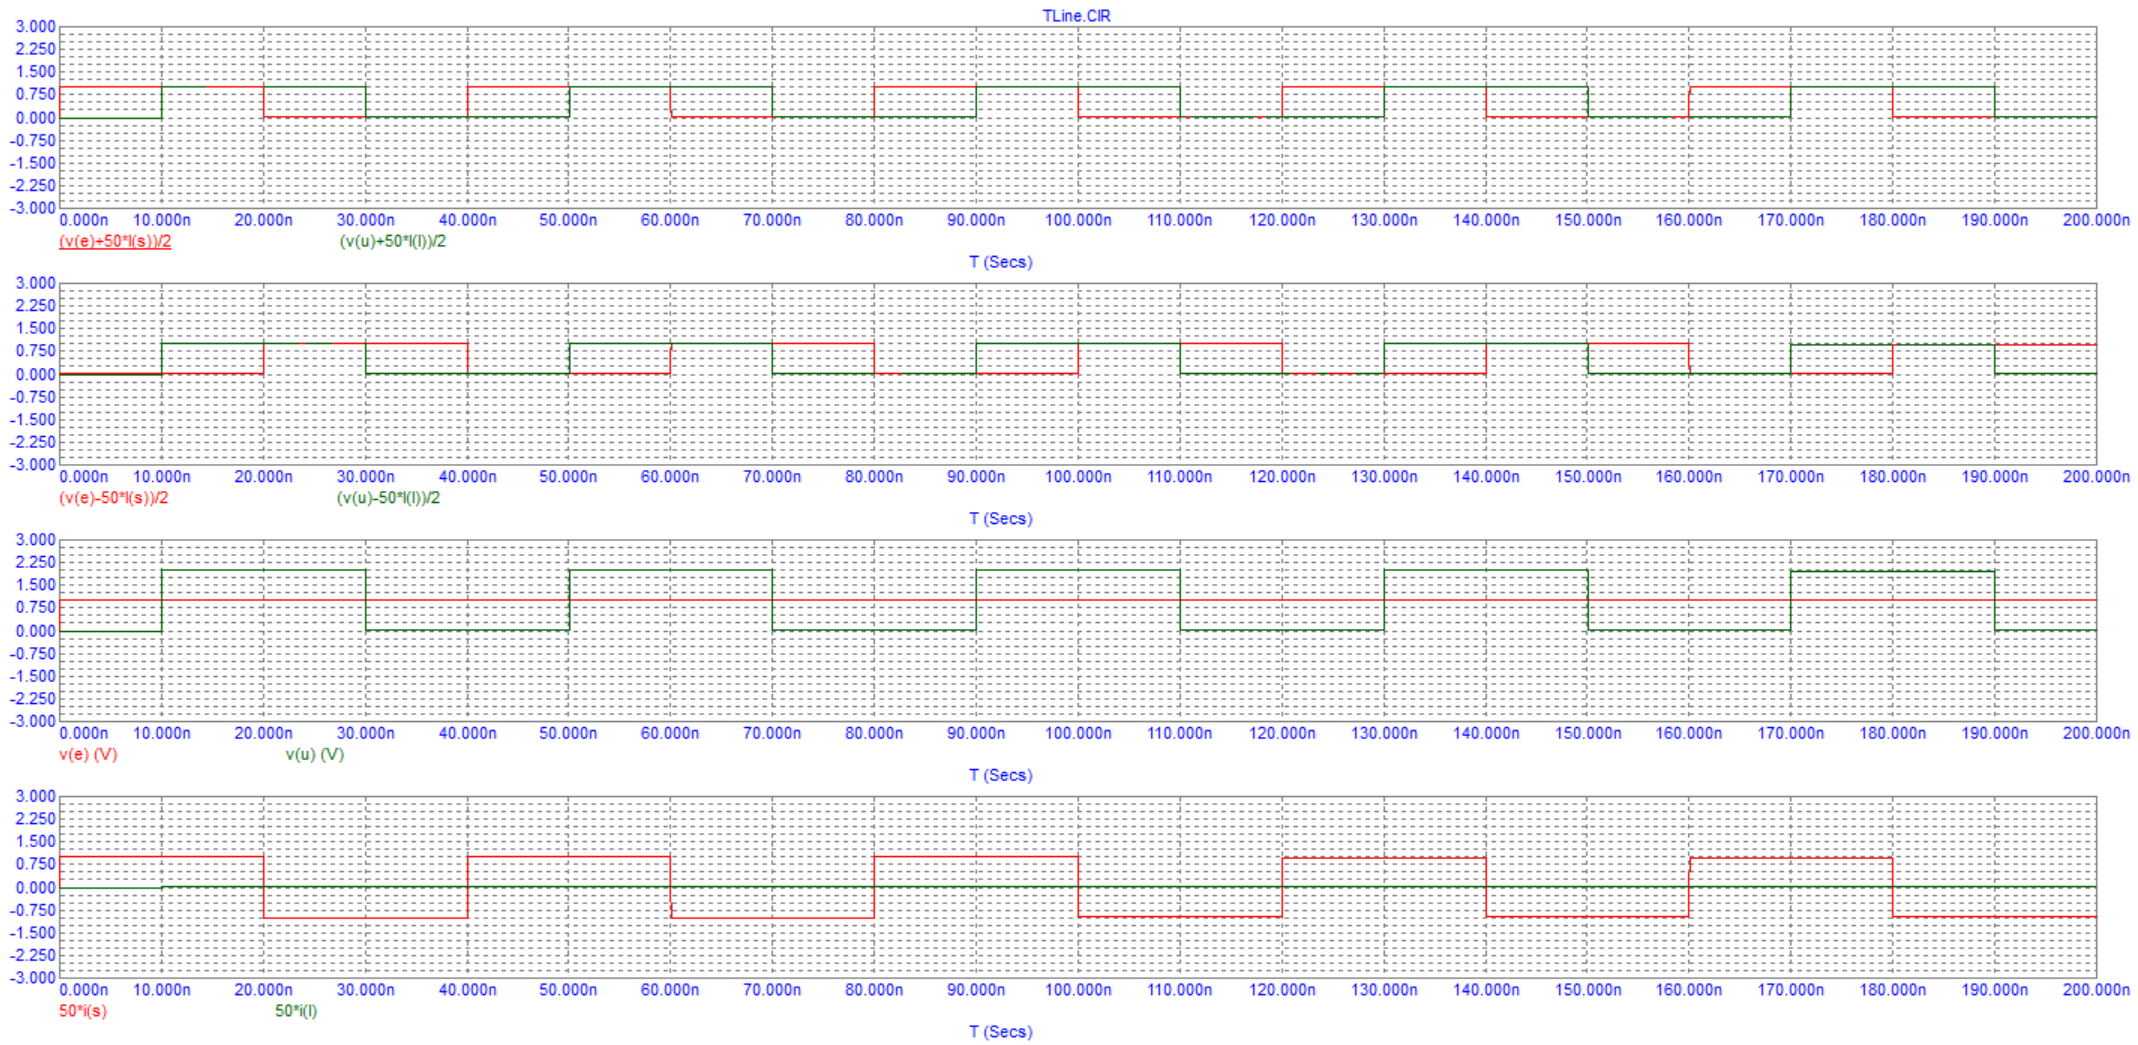
\includegraphics[width=0.95\textwidth]{картинки/Graph11.png}
\label{fig:Image1}
\caption{$R_l = 50k, R_s = 0$}
\end{figure}

.

\begin{figure}[h!]
\centering
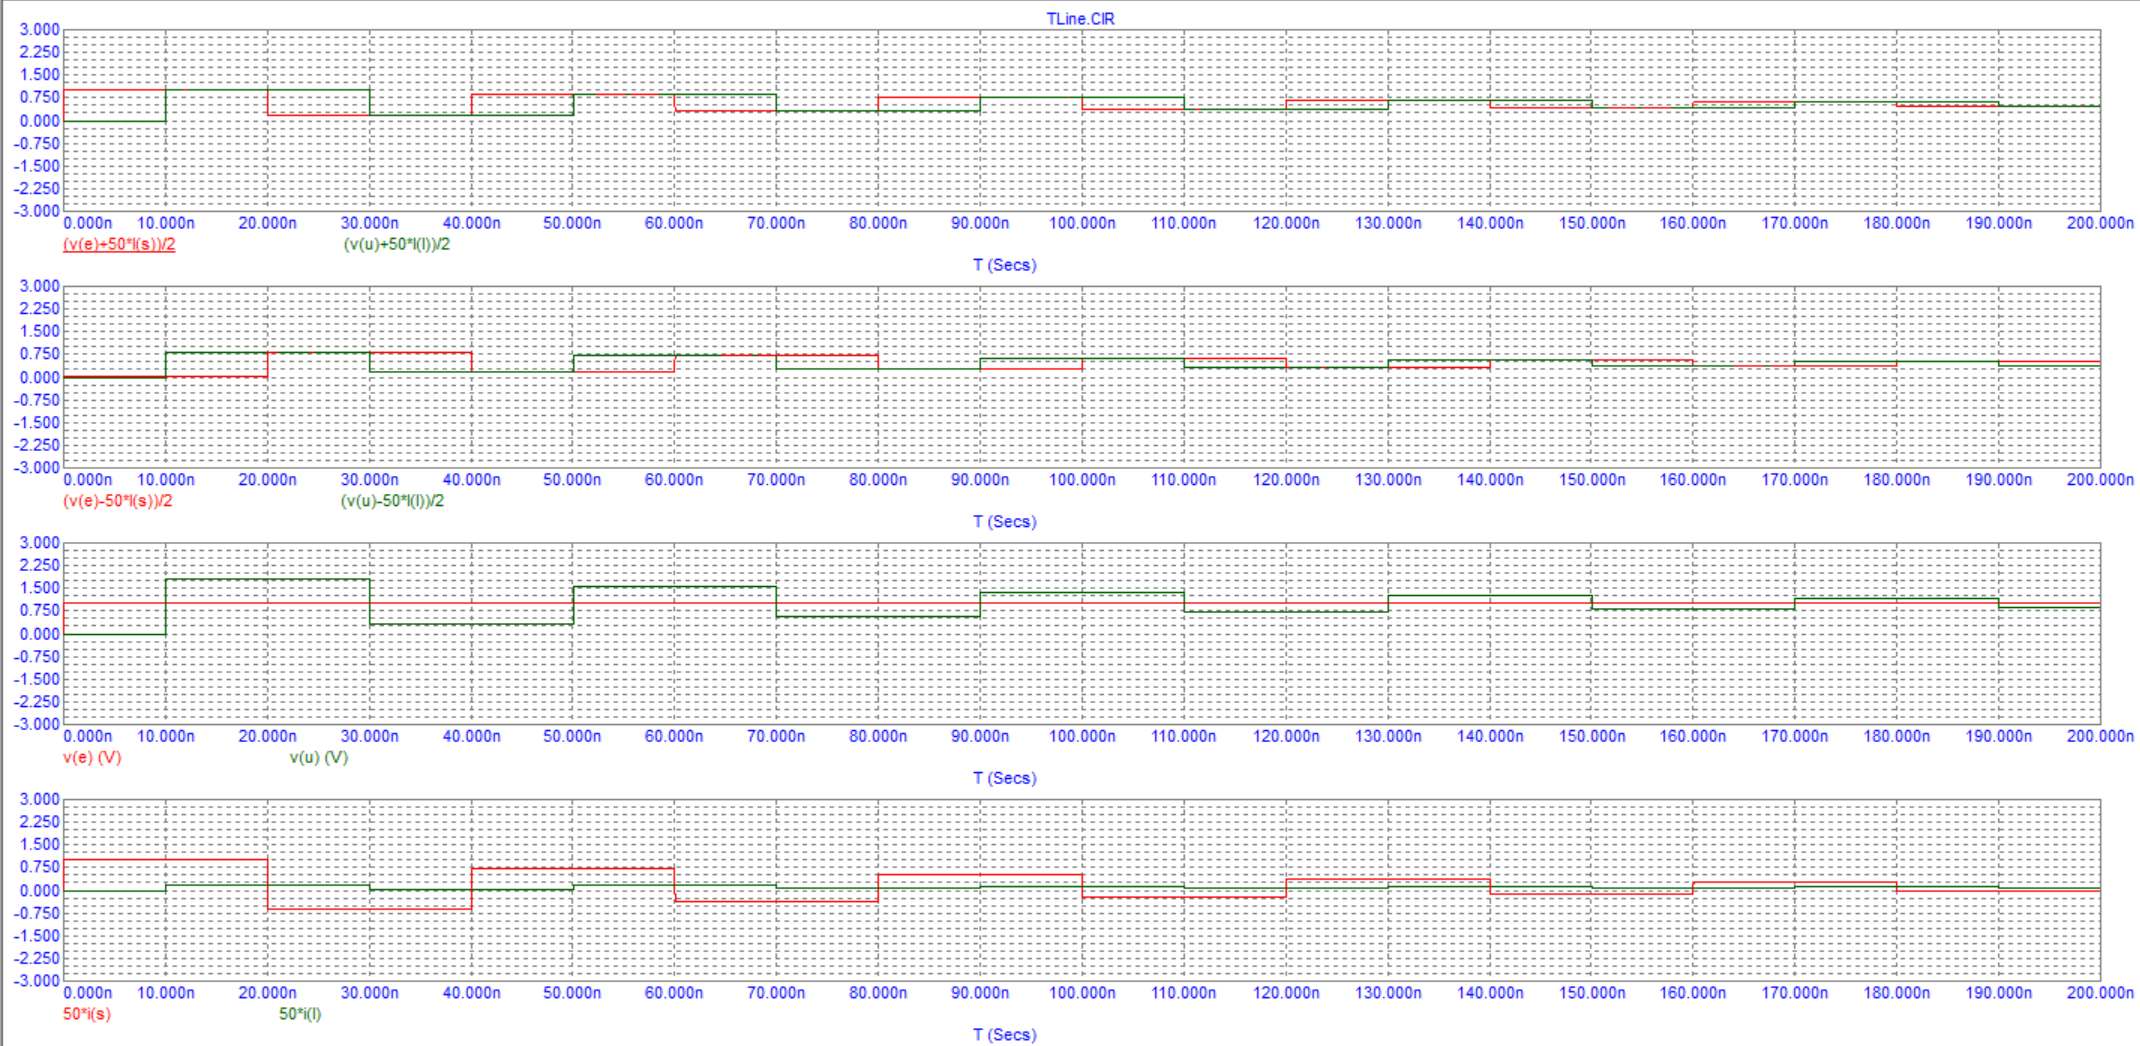
\includegraphics[width=0.95\textwidth]{картинки/Graph12.png}
\label{fig:Image1}
\caption{$R_l = 500, R_s = 0$}
\end{figure}

\newpage

\begin{figure}[h!]
\centering
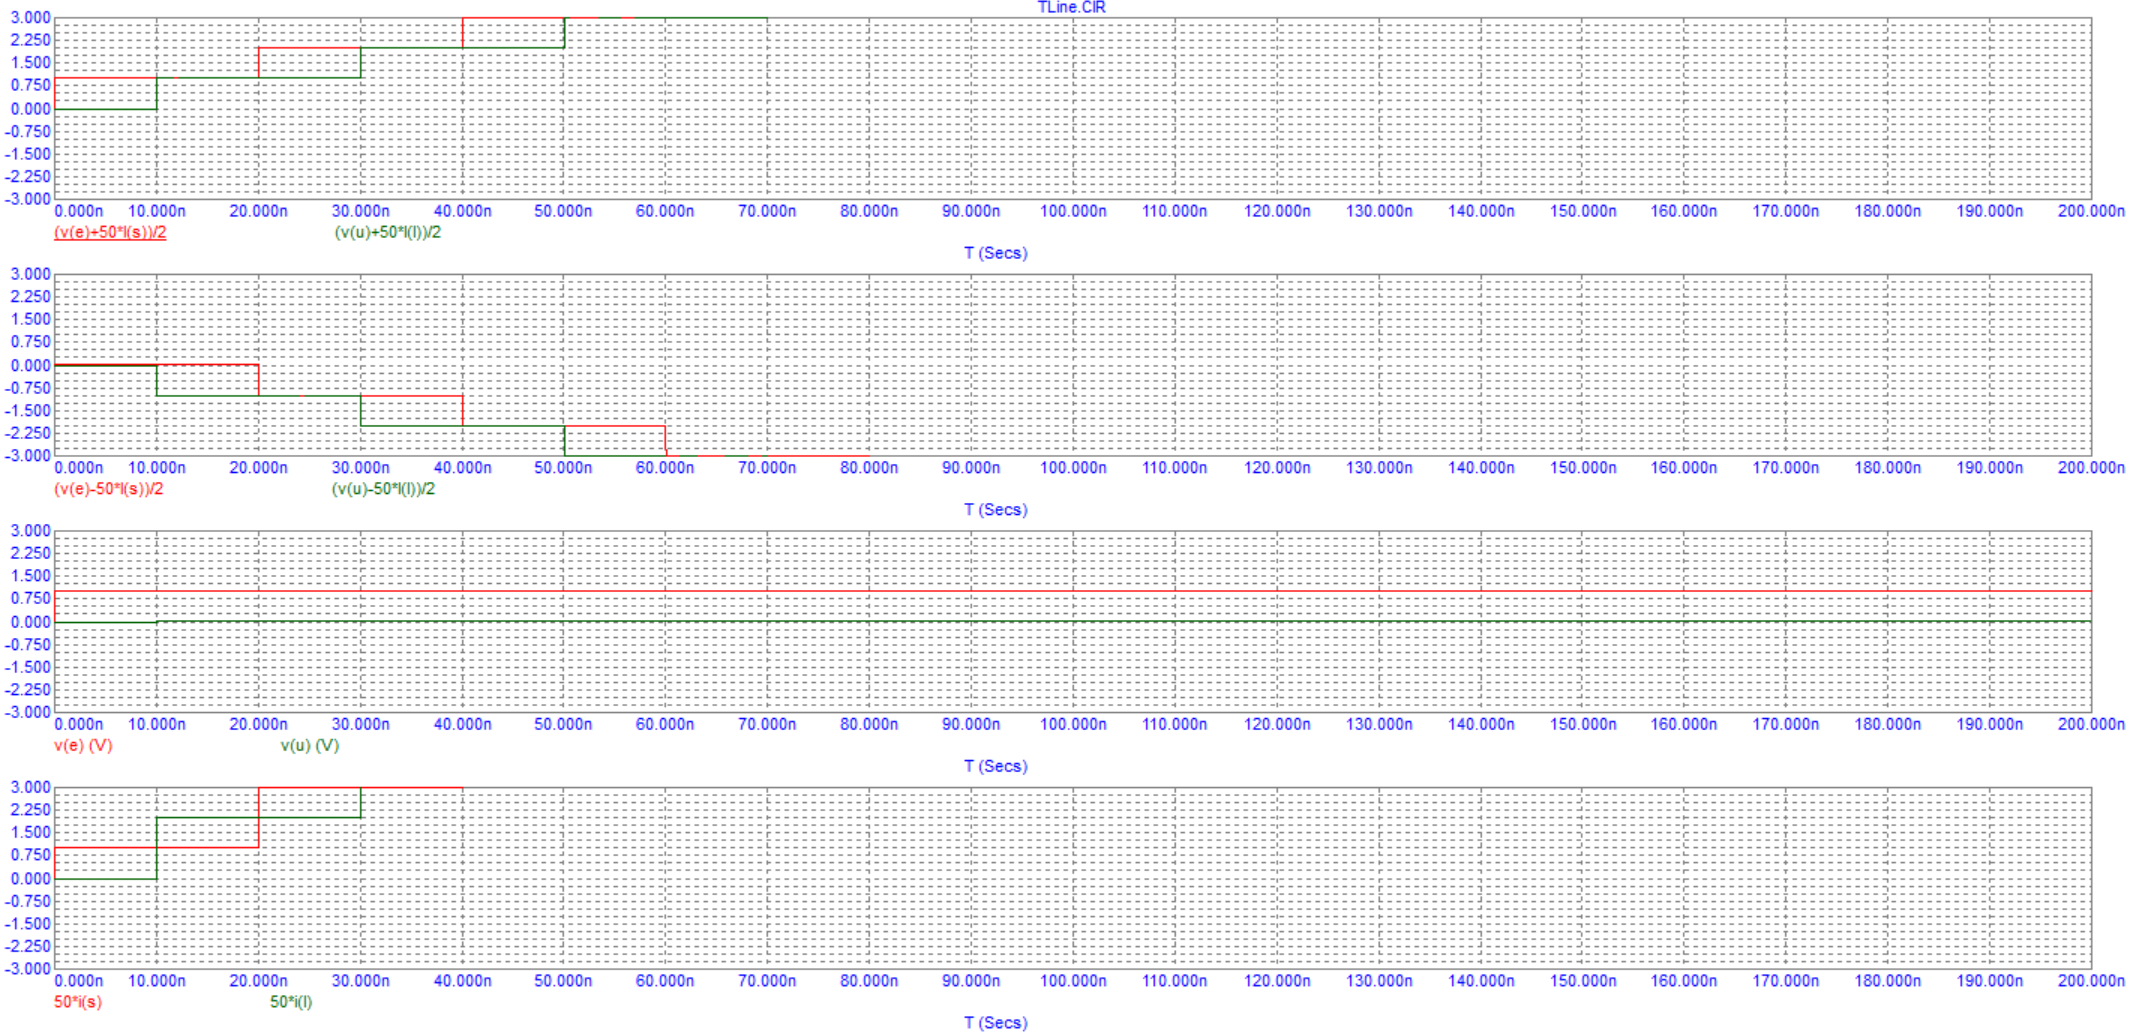
\includegraphics[width=0.95\textwidth]{картинки/Graph13.png}
\label{fig:Image1}
\caption{$R_l = 0, R_s = 0$}
\end{figure}

.

\begin{figure}[h!]
\centering
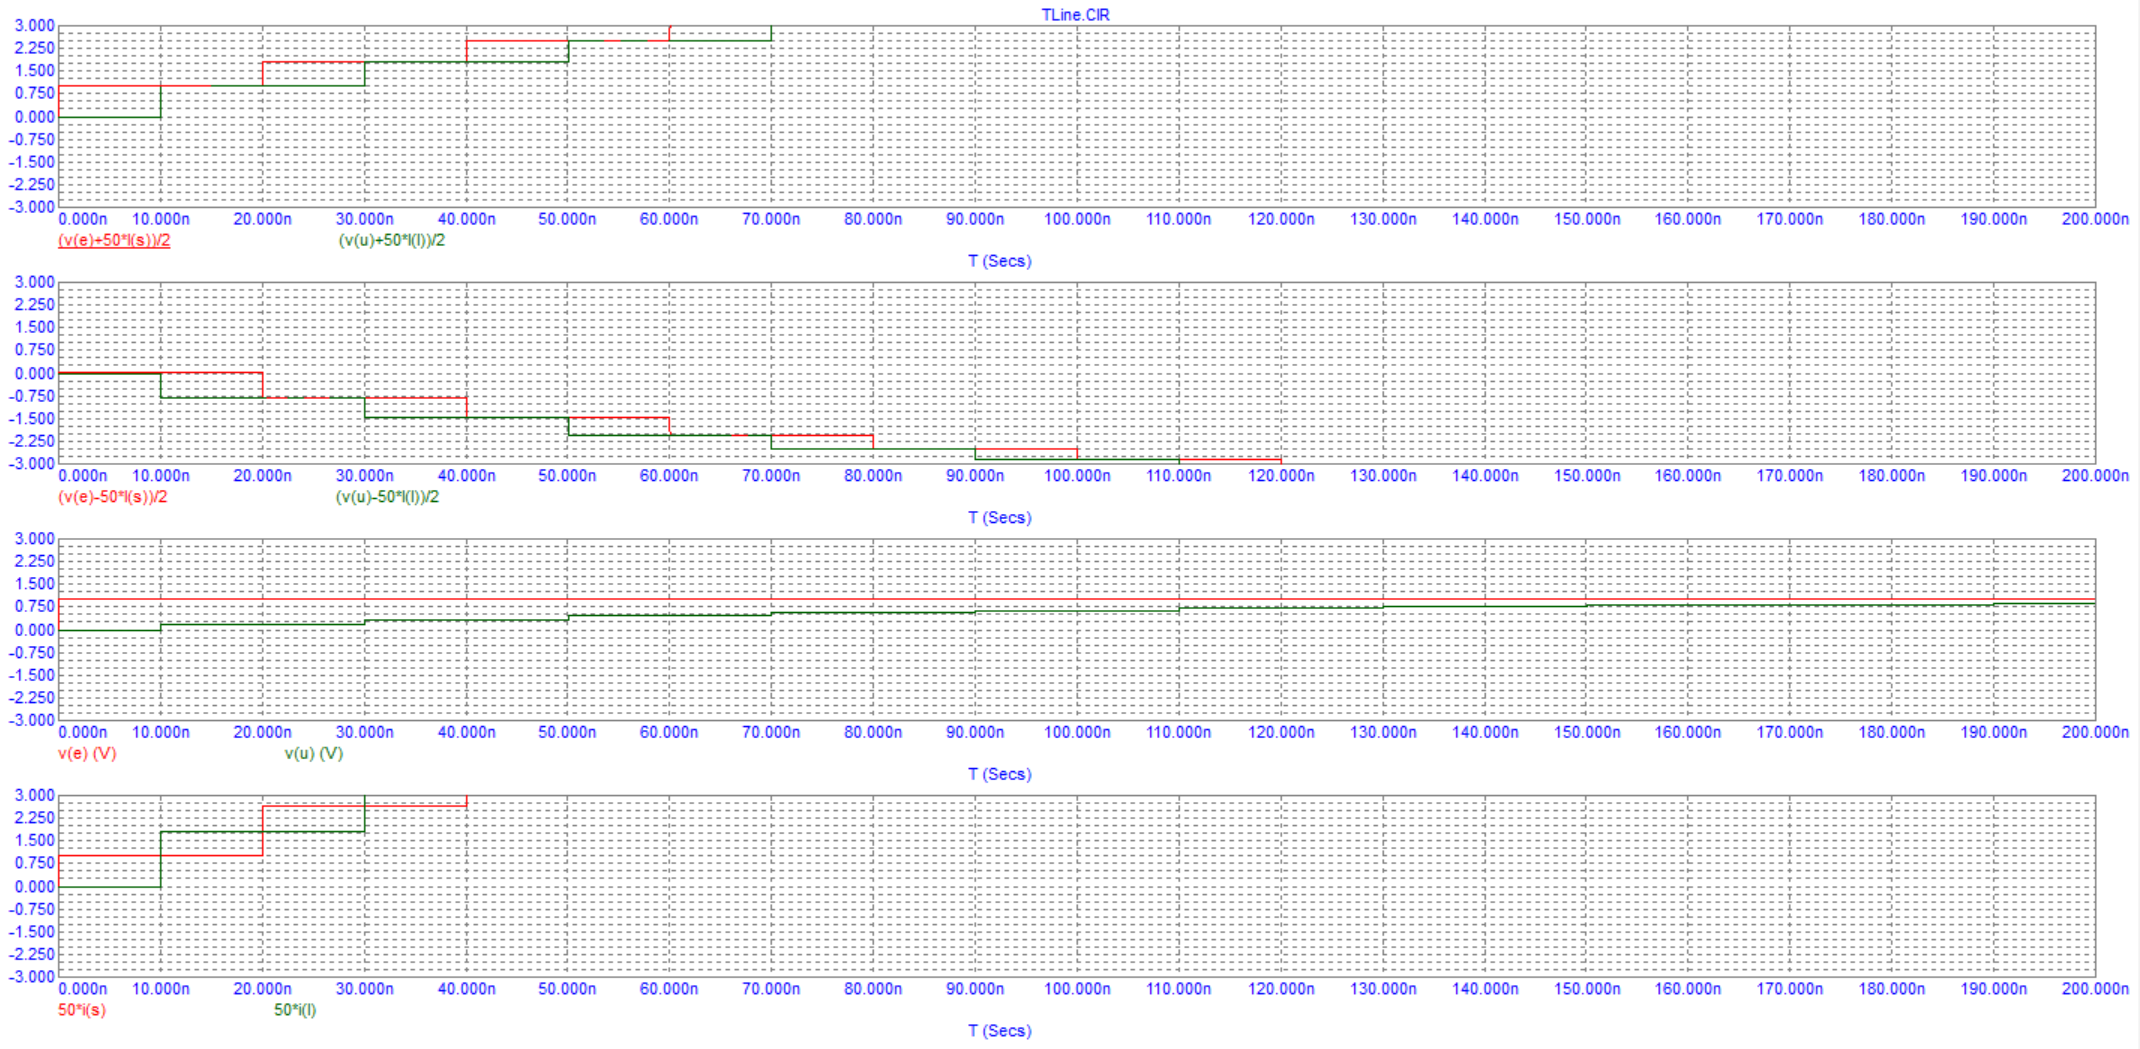
\includegraphics[width=0.95\textwidth]{картинки/Graph14.png}
\label{fig:Image1}
\caption{$R_l = 5, R_s = 0$}
\end{figure}

\newpage

\subsubsection{Емкостная нагрузка}

Установить на схеме $R_s = 50$ (согласованный источник), $R_l = 50k \simeq \infty, \: C = 100 \textit{ пФ}$.

\begin{figure}[h!]
\centering
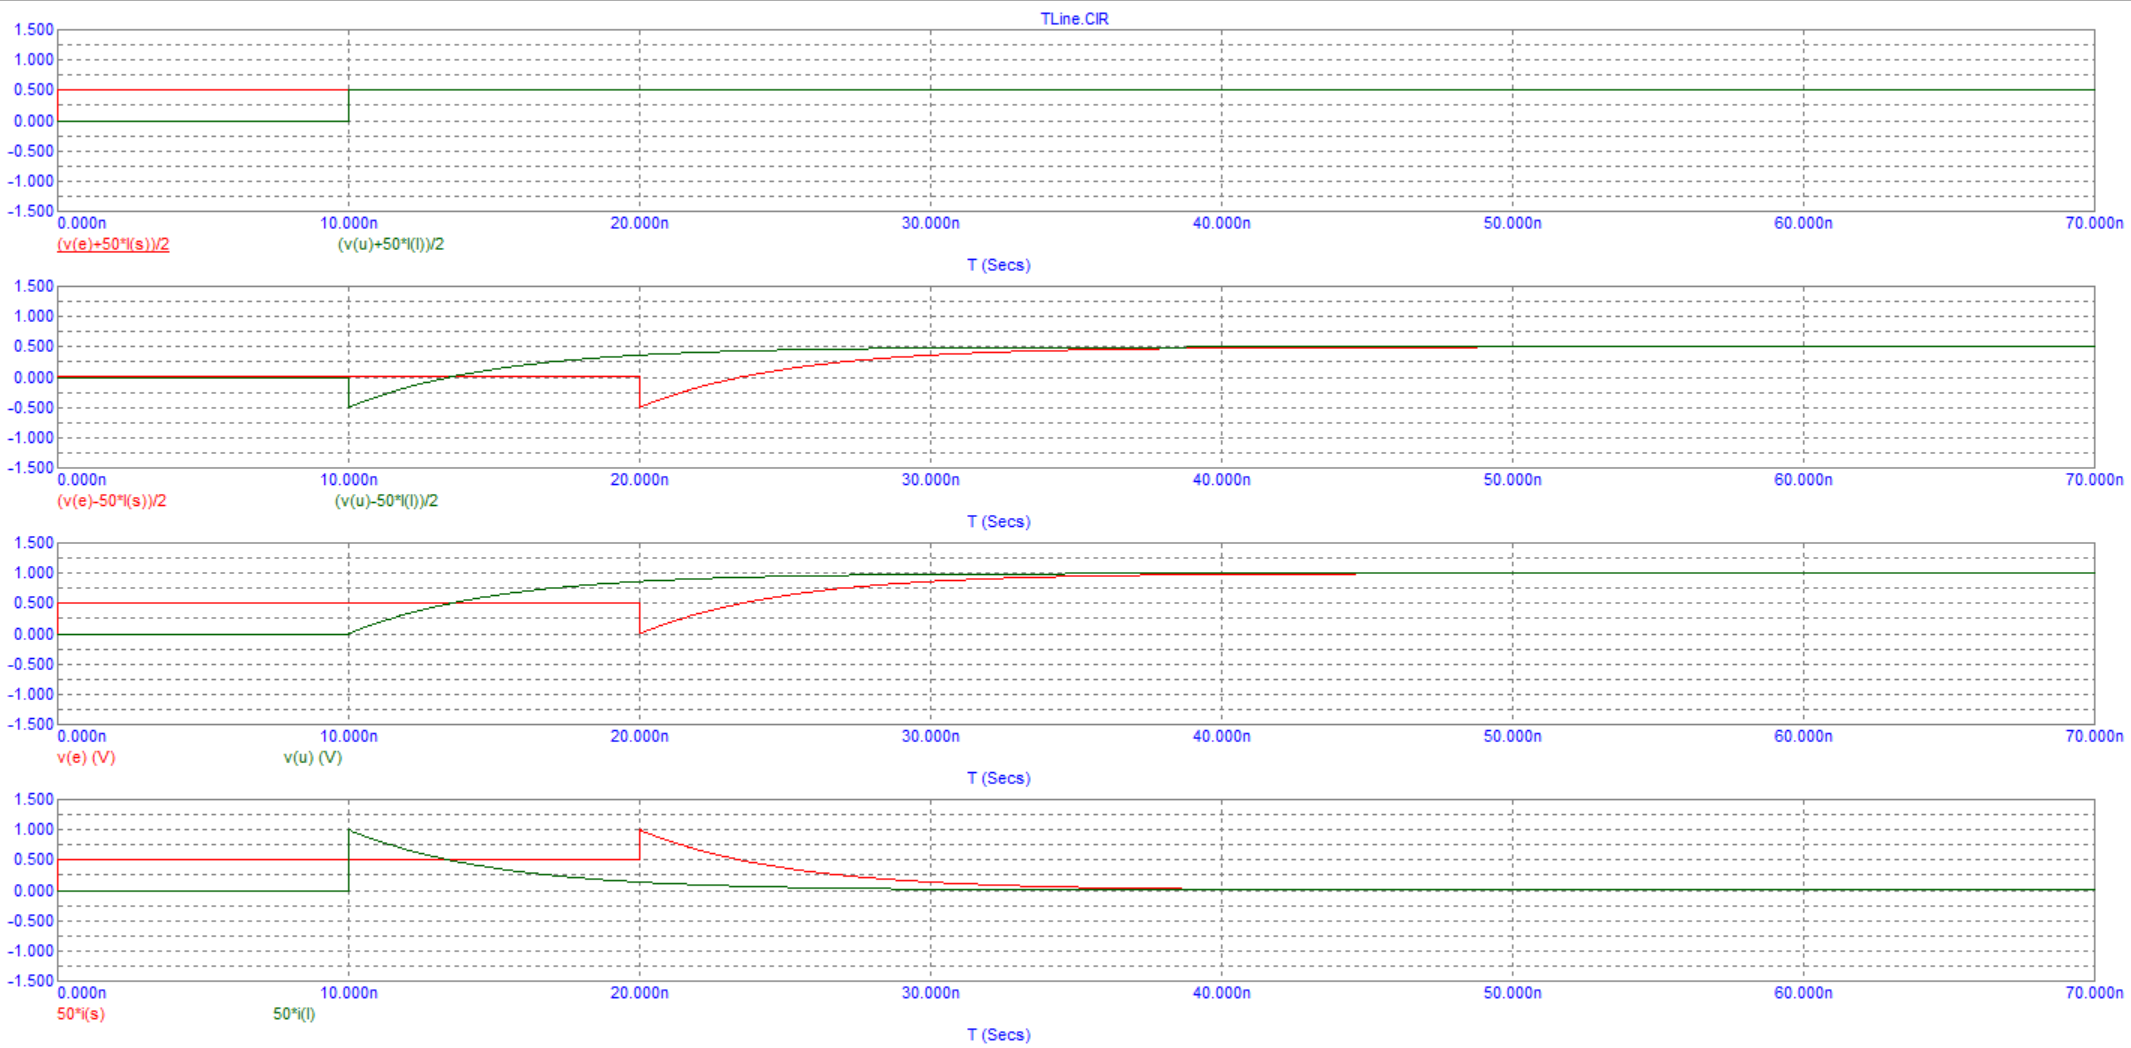
\includegraphics[width=0.95\textwidth]{картинки/Graph15.png}
\label{fig:Image1}
\caption{$R_l = 50k, R_s = 50$}
\end{figure}

Измерим установившееся значения амплитуд волн напряжений и токов:

\[A = 0.5 \: \textit{ В}\]

\[B = 0.5 \: \textit{ В}\]

\[u = 1 \: \textit{ В}\]

\[i\omega = 0 \: \textit{ В}\]

Оценим по графику постоянную времени $\tau$ экспоненциального переходного процесса:

\[u = u_0 \left(1 - \frac{1}{e}\right),\]

где $u_0 = 1 \: \textit{ В} \: \Rightarrow \: u = 0.63 \textit{ В}$, тогда:

\[\tau_{\text{эксп}} = 5.1 \: \textit{ нс}\]

\[\tau_{\text{теор}} = \omega C = 5 \: \textit{ нс}\]

Варьированием установим $R_s = 50/3$, проанализируем графики переходных процессов.

\begin{figure}[h!]
\centering
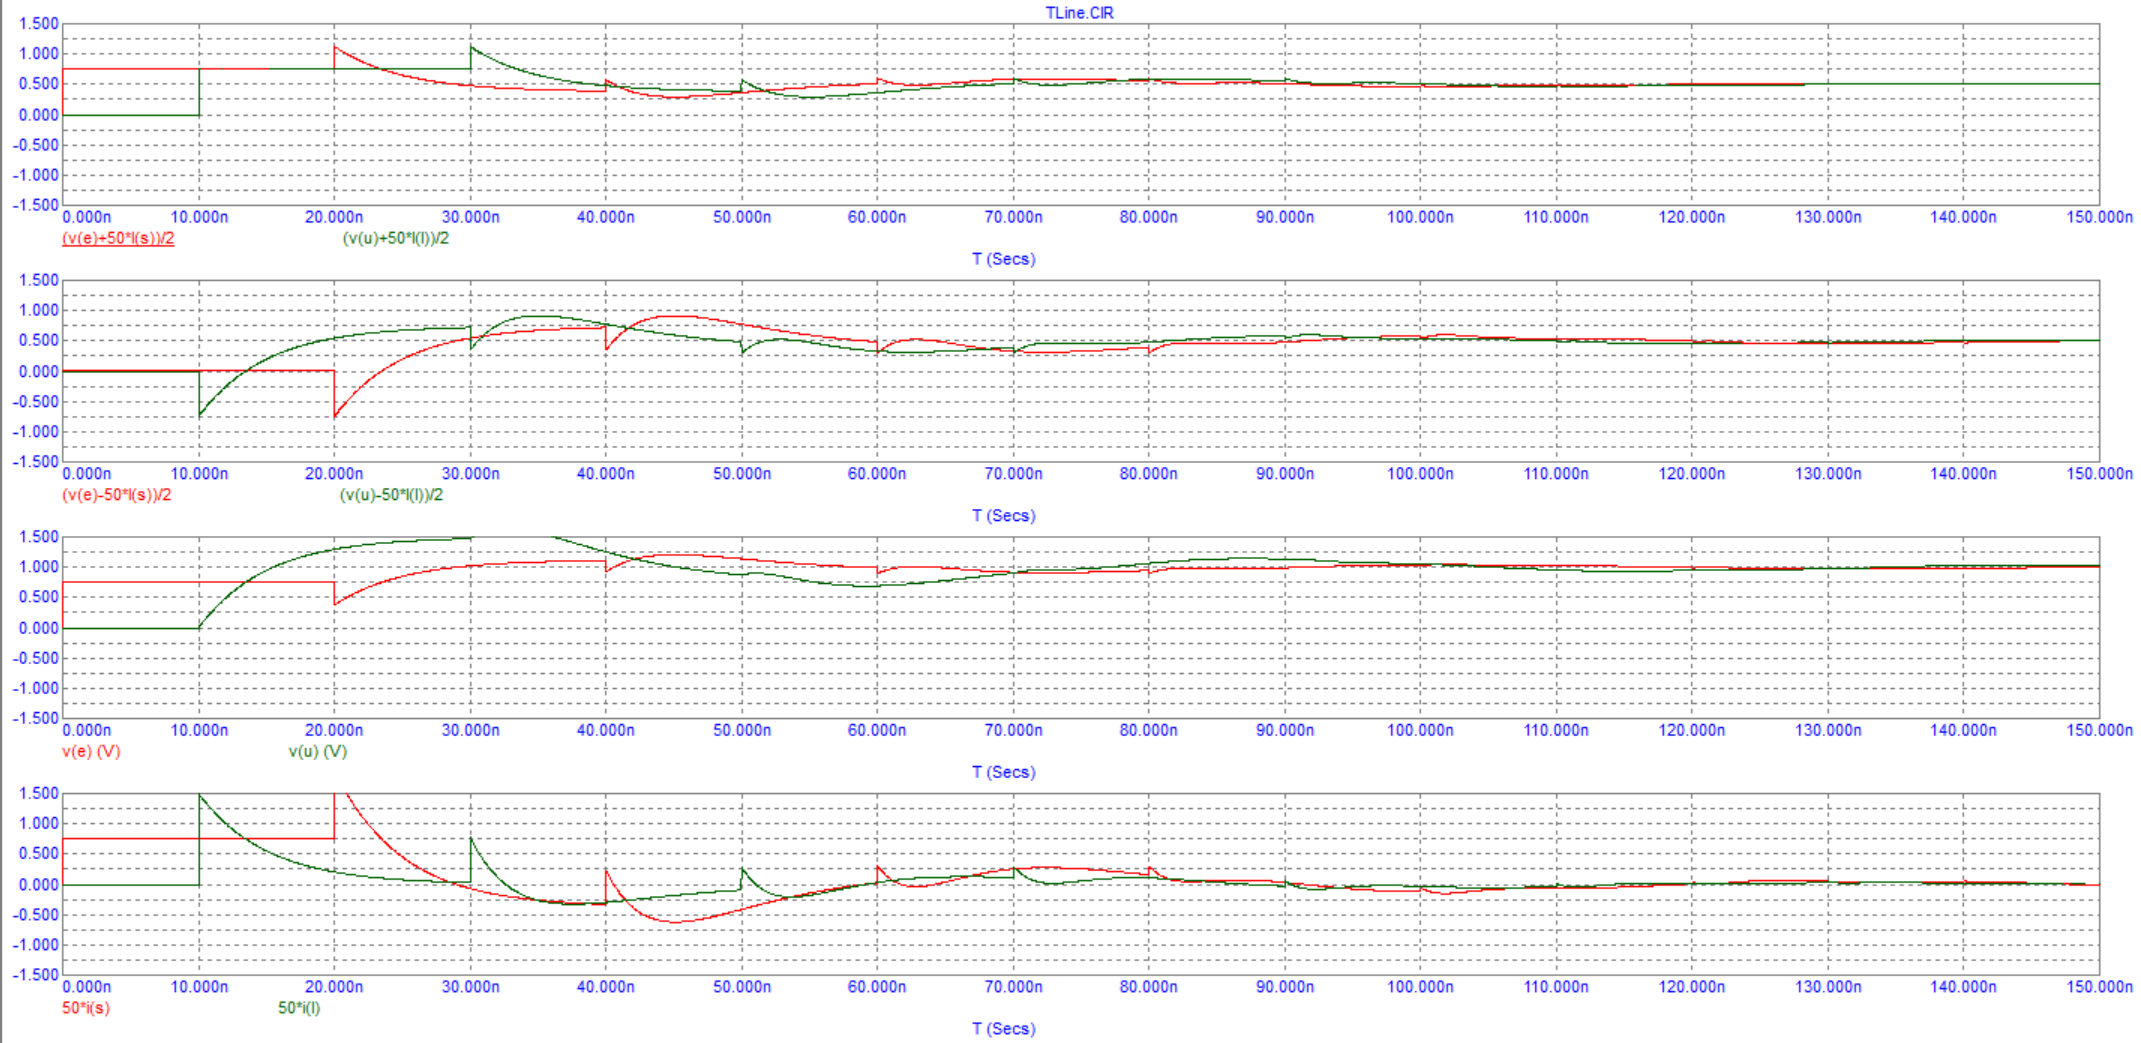
\includegraphics[width=0.95\textwidth]{картинки/Graph16.png}
\label{fig:Image1}
\caption{$R_l = 50k, R_s = 50/3$}
\end{figure}

\[A = 0.5 \: \textit{ В}\]

\[B = 0.5 \: \textit{ В}\]

\[u = 1 \: \textit{ В}\]

\[i\omega = 0 \: \textit{ В}\]

Проанализируем графики незатухающего переходного процесса при $R_s = 0$.

\begin{figure}[h!]
\centering
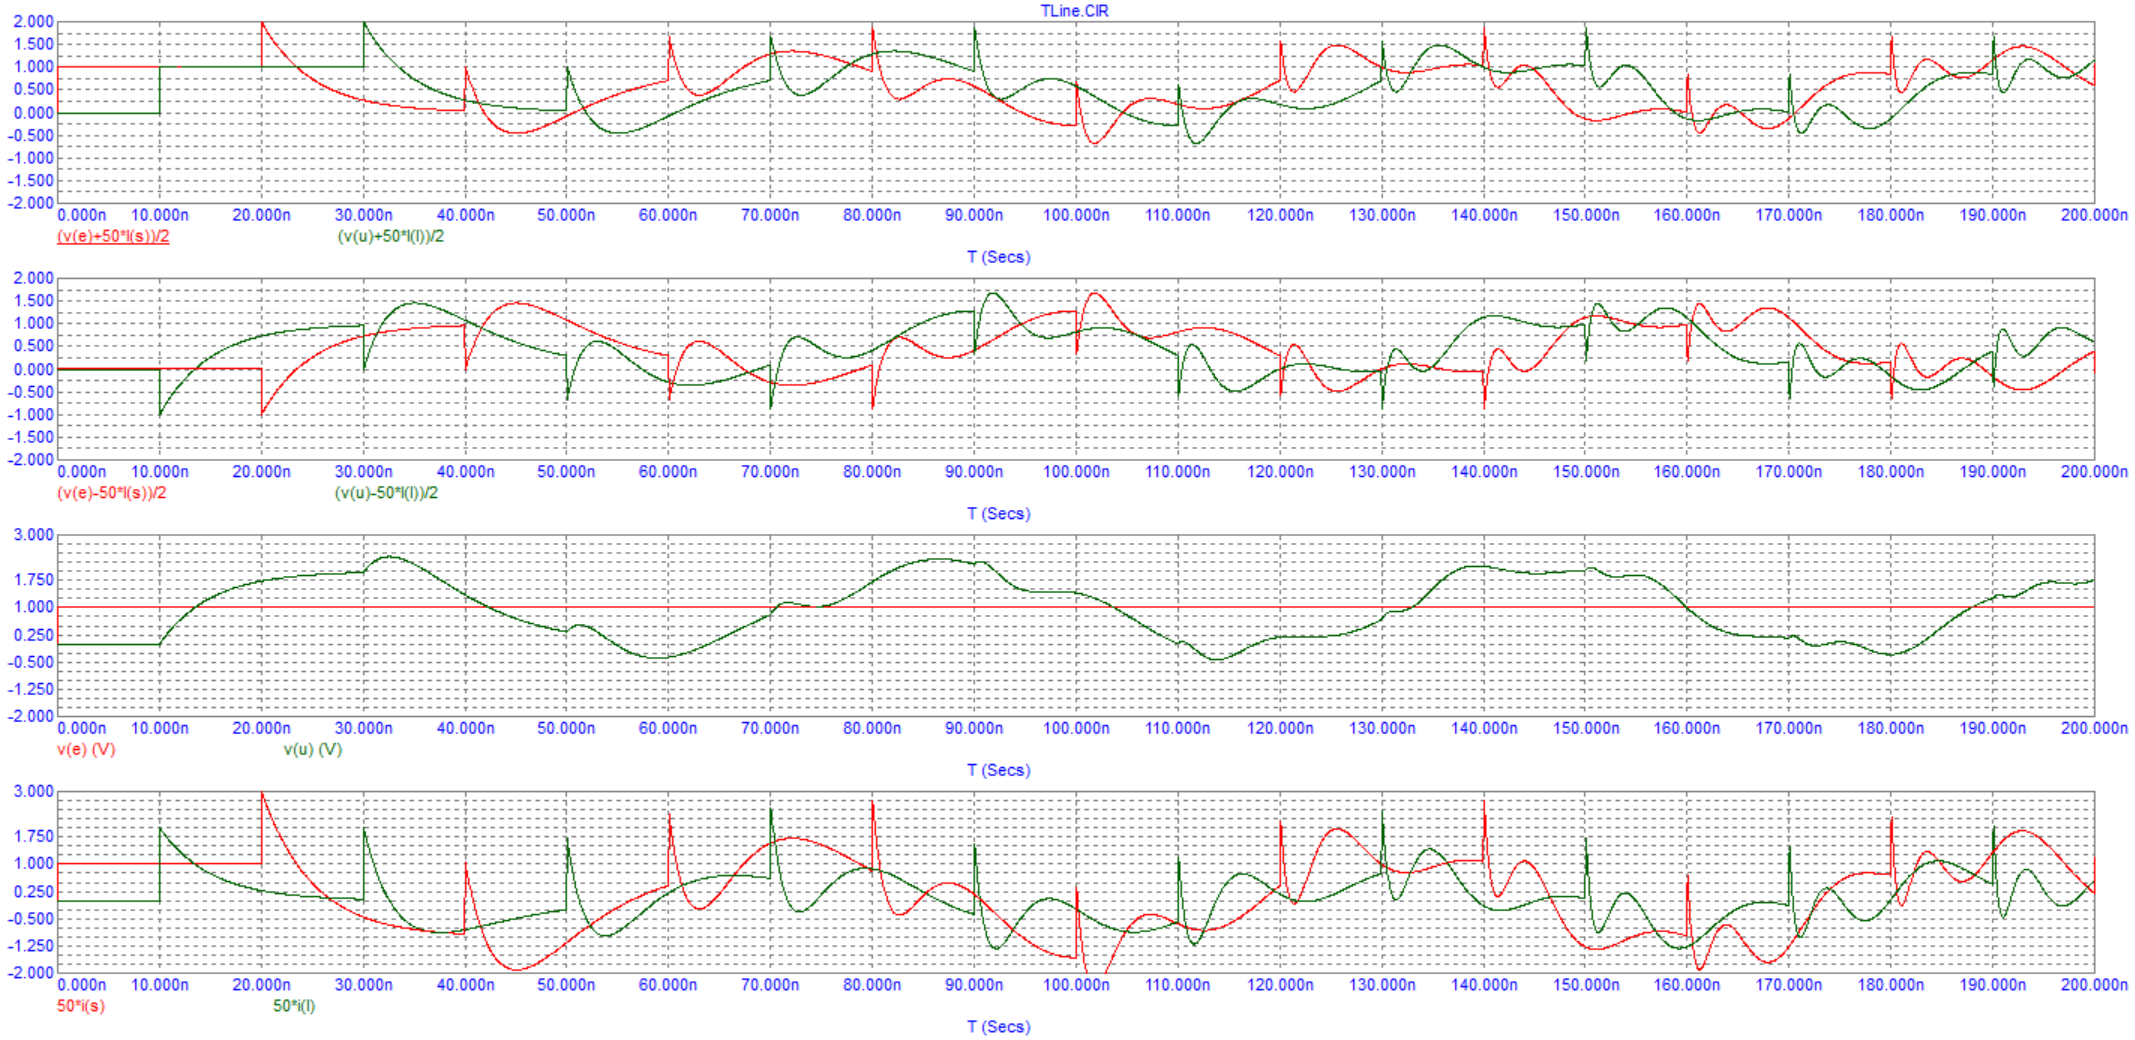
\includegraphics[width=0.95\textwidth]{картинки/Graph17.png}
\label{fig:Image1}
\caption{$R_l = 50k, R_s = 0$}
\end{figure}

\subsubsection{Вывод}

Моделирование полностью сходится с теорией, что вполне ожидаемо, разумно и естественно.

\section{Вывод}

Результаты моделирования, как и ожидается, тождественны теории, в то время как замеры на макетной плате незначительно от нее отличаются. Все это позволяет сказать, что использованные методы расчета и анализа безинерционных линейных цепей дают хорошие результаты в области применимости.


\end{problem}
\end{document}